\section{Axisymmetric Navier-Stokes Equations}
\subsection{Co-Ordinate Dimensions}

The use of axisymmetric co-ordinates can be used to great efficiency
when trying to solve a three dimensional problem.  The efficiency is manifested
by the reduction of the governing equations by one spatial dimension, thus 
reducing the complexity of the overall equation set and saving time in their 
solution.  By reducing a three dimensional problem to a two dimensional axisymmetric
problem, the computational domain is reduced by orders of magnitude through the 
addition of a source term similar in thought to that of the source 
term for \emph{Quasi-2D flow}.  

However, it should be noted that unlike \emph{Quasi-2D flow} 
where a two dimensional flow is approximated as having only one dimension (for example, 
inviscid flow through a converging nozzle can be described as having velocity only along the 
length of the nozzle despite the fact that there must be some normal velocity for the flow
to follow the nozzle contour), axisymmetric flow is really only a special type of \emph{three}
dimensional flow, and hence not, in fact, a \emph{Quasi-2D flow}.  This point is best 
illustrated by the fact that the shock angles on an infinte wedge and cone are different, this 
difference being a direct result of the three dimensional nature of the flow around a cone.

\begin{figure}[h]
\begin{center}
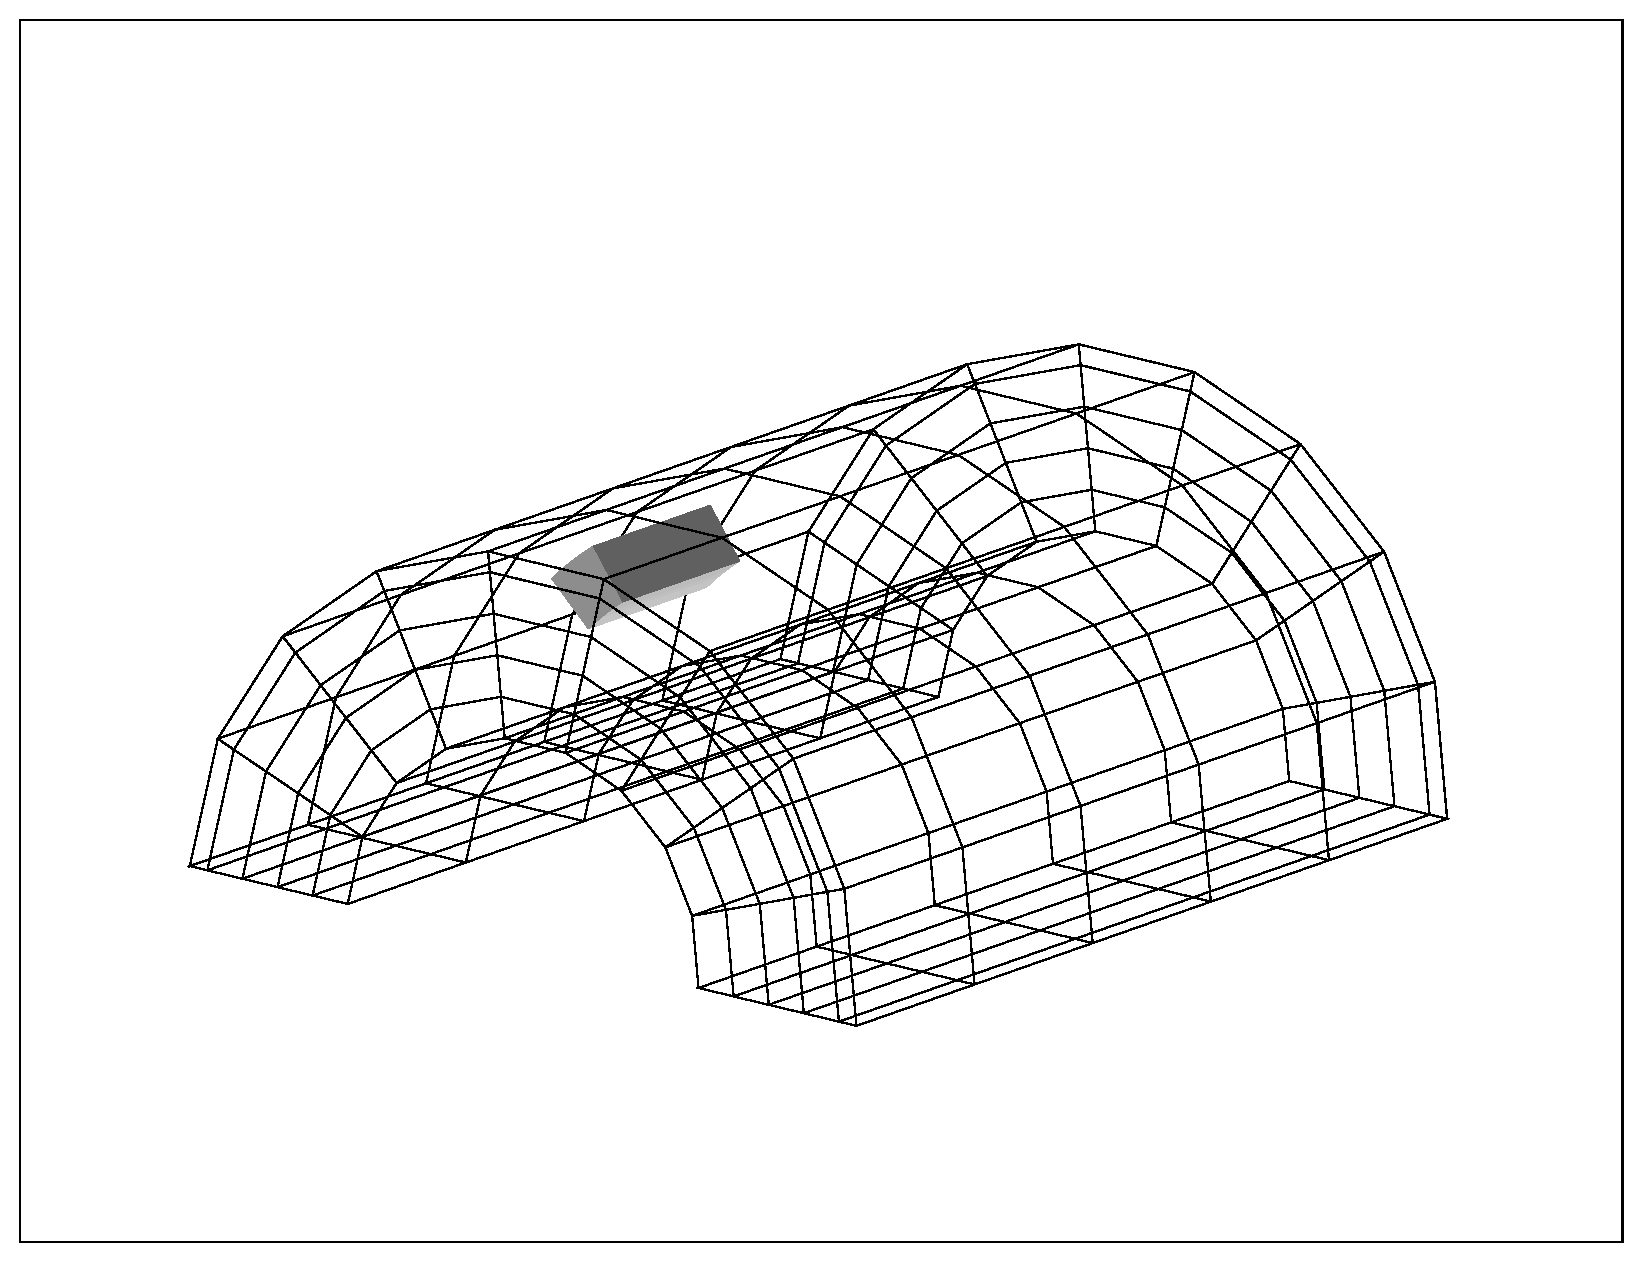
\includegraphics[width=5cm]{./cyl_grid.eps}
% One can specify [angle=x,width=y,height=z] for the graphics
\caption{Axisymmetric Grid Space}
\label{fig:grid}
\end{center}
\end{figure}

\indent In order to derive the axisymmetric Navier-Stokes equations, let us examine 
in detail an axisymmetric flow field. Fig. \ref{fig:grid} shows a half portion of a
generic axisymmetric domain, with an infantesimal region shaded within.  In order to reduce the 
computational effort required to solve a given scenario, it is convenient to express the problem 
in only two co-ordinate directions and account for the three dimensional effects through the use of
a source term.  For this approach to be correct, the flow field must be accuractly described
by a planar set of variables that can be taken to exist at any location in the circumferential
direction ($\theta$ axis).  Mathematically this condition is expressed by the following relation,

\begin{equation}
	\frac{\partial}{\partial \theta}=0 
\label{eqn:dtheta}
\end{equation}

	By further restricting the problem to a set of flow variables where the circumferential
velocity is taken as zero ($w = 0$) this eliminates the need to consider any variables in the out of plane 
dimension.  This has the effect of reducing the $\theta$ dimension to a 'void'
dimension, one that contains no flowing properties but has a physical presence in that one still
considers an infantesimal \emph{volume} when deriving the appropriate equations (also, as
will be seen in subsequent sections on turbulence, one must consider flow velocity in 
the circumferential direction for the purposes of deriving a set of axisymmetric equations,
despite the fact that the resulting equations will not contain this variable explicitly).  As well,
forces acting on the faces of the 'void' dimension must still be carefully considered as they
can in certain instances exert an influence the radial ($r$ axis) direction.  This approach is 
similar to that used when deriving a set of \emph{Quasi-2D} equations, where one makes use of 
an infantesimal	area but restricts flow variables to the first co-ordinate axis only (in essence 
creating a 'void' dimension).

	At first glance this approach may seem to contain an inconsistency in that, for example, 
in the case of supersonic flow over a cone the axisymmetric equations are able to accurately predict 
what is sometimes referred to as the three dimensional relieving effect (the reduction of the 
shock angle on a cone when compared to a wedge with an angle equal to the half angle of the cone). 
This effect is created by the fact that the flow is able to expand not only in the radial and 
axial directions, but the circumferential direction as well.  However, expansion along the 
circumferential axis by definition requires that the flow be allowed to travel in this direction, 
which as previously stated is not permitted as this dimension is declared 'void'.  

	The key to resolving this paradox lies in remembering that the Navier-Stokes equations 
deal with flows as a continuum, and as a result necessarily rely on the averaging of molecular
processes.  From a molecular viewpoint, as each particle travels along the cone it's tendency
to deviate from it's original $x$-$r$ plane is equally as likely to be left as it is to be right.  
Thus on average,for each particle traveling on a given ray that deviates to the left, 
there exists another particle traveling along this ray that deviates to the right.  This explains
why upon averaging the molecular movements, which is the basis for the Navier-Stokes equations, 
one sees no apparent movement in the circumferential direction while still being able to account
for the expansion of the flow in this direction.  

%-------------------------------------------------------------------------------------------------------------
\subsection{Species Conservation}

\begin{figure}[!h]
\begin{center}
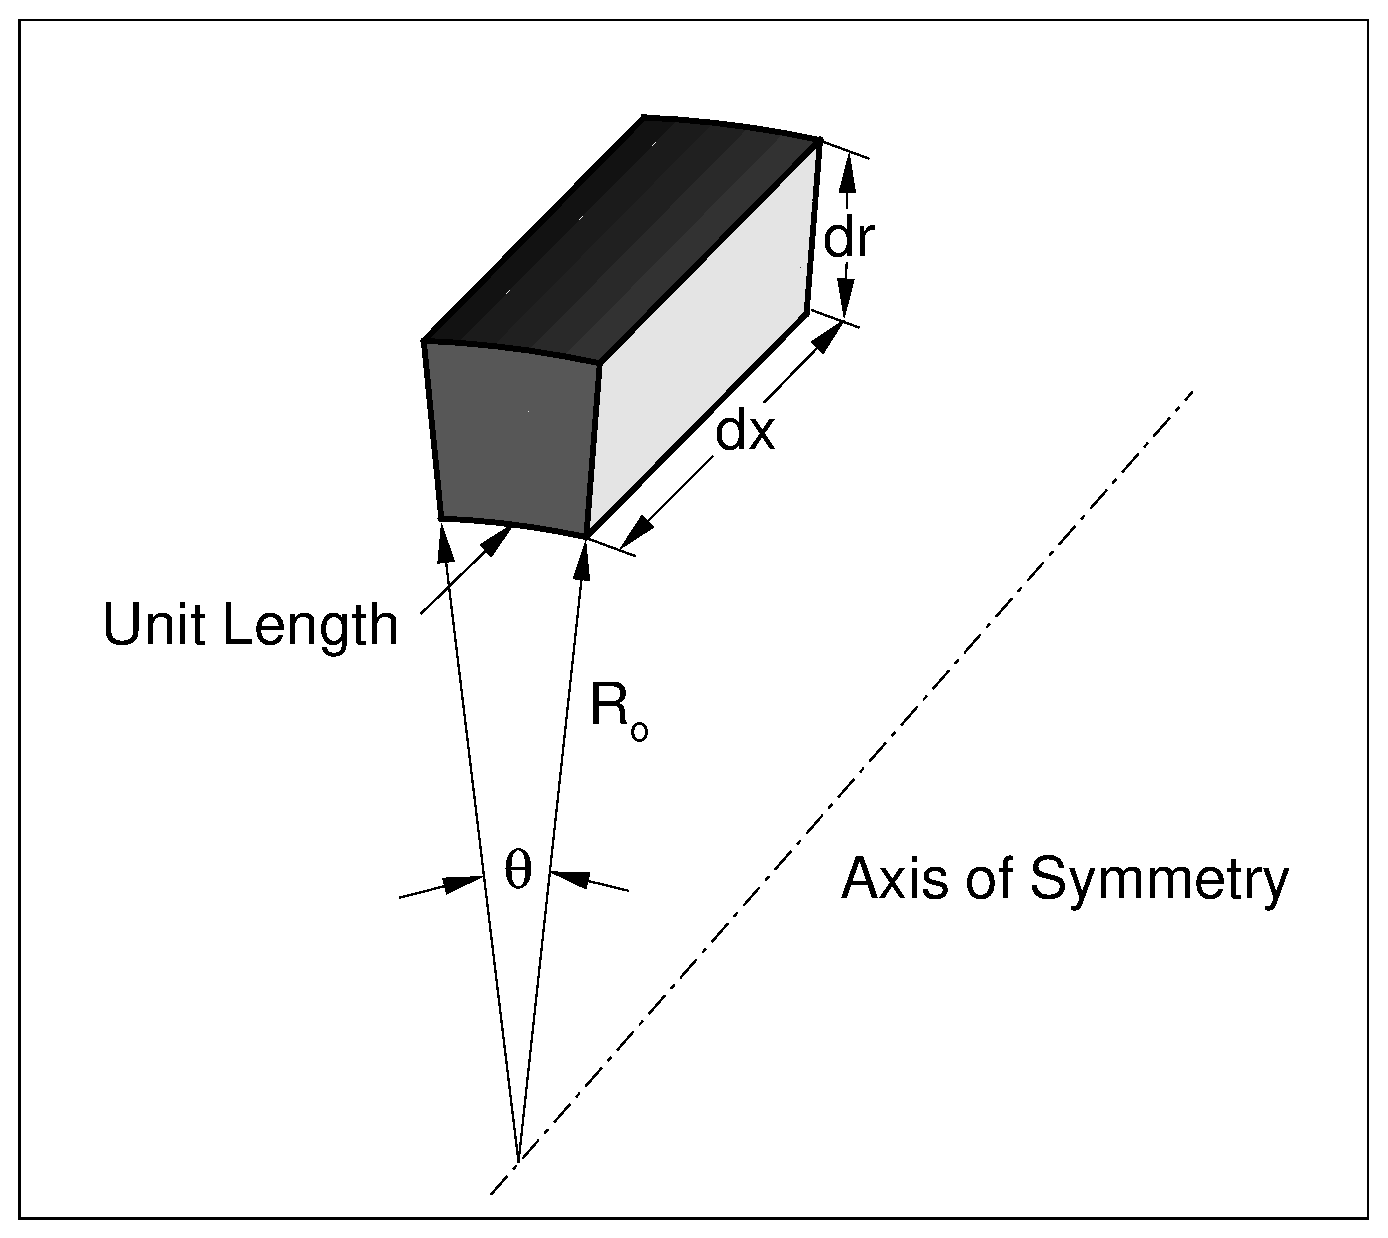
\includegraphics[width=5cm]{./infantesimal.eps}
% One can specify [angle=x,width=y,height=z] for the graphics
\caption{Infantesimal Axisymmetric Volume}
\label{fig:inftes}
\end{center}
\end{figure}

	In order to derive the conservation of mass equations for a multi-species flow, let us 
consider the infantesimal volume shown in Fig. \ref{fig:inftes}.  As can be seen, although the
equations to be derived will be for planar flow (and hence be valid in any $x$ - $r$ plane),
the fluid volume used to obtain these equations must be appropriately defined to account for the
curved nature of the $\theta$ dimension.  In this derivation, the desired
equation will be derived by considering the behaviour of the flow along each co-ordinate direction
separately and then combining the results to arrive at the final equation.



%-------------------------------------------------------------------------------------------------------------------------
\subsubsection{$x$ direction}

\begin{figure}[ht]
\includegraphics[height=5cm]{./xdir.eps}
% One can specify [angle=x,width=y,height=z] for the graphics
\caption[$r$ - $\theta$ planes]{$r$ - $\theta$ planes : All fluid properties are depicted by solid lines while 
				forces acting on the infantesimal fluid element are depicted by dashed lines (these include
				the pressure acting on the front an back $r$ - $\theta$ planes, as well as the shear
				acting on the $x$ - $r$, $x$ - $\theta$, and $r$ - $\theta$ planes)}
\label{fig:xdir}
\end{figure}

\begin{displaymath}
	\begin{array}{ccc}
		\begin{array}{c}
			\textrm{Mass flow of species \emph{k}} \\ \textrm{in through the front $r$ - $\theta$ plane} 
		\end{array} & 
	= & (\rho_k u)dr(R_o \theta) + j_{k_x} dr(R_o \theta)\\
	& \\ & \\
		\begin{array}{c}
			\textrm{Mass flow of species \emph{k}} \\ \textrm{out through the back $r$ - $\theta$ plane}
		\end{array} & 
	= & \begin{array}{c}
		(\rho_k + \frac{\partial \rho_k}{\partial x}dx)(u + \frac{\partial u}{\partial x}dx)dr(R_o \theta) \\
	+ (j_{k_x} + \frac{\partial j_{k_x}}{\partial x}dx)dr(R_o \theta)
		\end{array}
	\end{array}
\end{displaymath}

	In the above equations, $j_{k_x}$ is the diffusive flux caused by gradients existing in the concentration
of species \emph{k}, which give rise to movement of the given species in the direction opposite the gradient
(Note that $j_{k_x}$ has units of $kg/m^2 s$). All other terms are shown in Fig. \ref{fig:xdir}.
Taking the difference between these two planes (outflow - inflow) yields,

\begin{displaymath}
	\Delta \dot{m}_{k_x} = \Big\{(\rho_k u + j_{k_x} + \rho_k \frac{\partial u}{\partial x}dx + u \frac{\partial \rho_k}
	{\partial x}dx + \frac{\partial u}{\partial x} \frac{\partial \rho_k}{\partial x}dx^2 + \frac{\partial j_{k_x}}
	{\partial x}dx) - (\rho_k u + j_{k_x})\Big\} dr(R_o \theta)
\end{displaymath}

	Canceling like terms, neglecting any resulting triple products of differential quantities, and collecting terms
using the inverse of the chain rule (from the Calculus) to combine derivatives yields the following,

\begin{displaymath}
	\Delta \dot{m}_{k_x} = \Big( \frac{\partial \rho_k u}{\partial x} + \frac{\partial j_{k_x}}{\partial x}
	\Big)dxdr(R_o \theta)
\end{displaymath}
 
	It should be noted that here, and in all subsequent derivations, the area used for quantities passing through
the infantesimal volume in the $x$ direction is simply $dr(R_o \theta)$.  This assumes that the two sides of
the volume (the boundary $x$ - $r$ planes) are parallel, which is not the case as can be seen in Fig. \ref{fig:xdir}.
By making this assumption, one neglects a pie shaped area of the $r$ - $\theta$ plane, which if approximated by a 
triangle, can be calculated as,

\begin{displaymath}
	\begin{array}{ccc}
		\textrm{Area} & = & \frac{1}{2}bh \\
		\textrm{Area} & = & \frac{1}{2}\Big\{\theta(R_o + dr) - \theta(R_o)\Big\}(dr) \\
		\textrm{Area} & = & \frac{1}{2}\theta dr^2
	\end{array}
\end{displaymath}

	With the neglected area defined one can calculate the flow properties through this area as was done
previously, using $\rho_k$ as an example

\begin{displaymath}
	\begin{array}{ccc}
		\begin{array}{c}
			\textrm{Mass flow of species \emph{k}} \\ \textrm{in through the neglected area} 
		\end{array} & 
	= & (\rho_k u)(\frac{1}{2}\theta dr^2) + j_{k_x} (\frac{1}{2}\theta dr^2)\\
	& \\ & \\
		\begin{array}{c}
			\textrm{Mass flow of species \emph{k}} \\ \textrm{out through the neglected area}
		\end{array} & 
	= & \begin{array}{c}
		(\rho_k + \frac{\partial \rho_k}{\partial x}dx)(u + \frac{\partial u}{\partial x}dx)
		(\frac{1}{2}\theta dr^2) \\
	+ (j_{k_x} + \frac{\partial j_{k_x}}{\partial x}dx)(\frac{1}{2}\theta dr^2)
		\end{array}
	\end{array}
\end{displaymath}

	Again taking the diffence between the outflow minus the inflow yields,

\begin{displaymath}
	\Delta \dot{m}_{k_{\textrm{Area}}} = \Big\{(\rho_k u + j_{k_x} + \rho_k \frac{\partial u}{\partial x}dx 
					     + u \frac{\partial \rho_k}
	{\partial x}dx + \frac{\partial u}{\partial x} \frac{\partial \rho_k}{\partial x}dx^2 + \frac{\partial j_{k_x}}
	{\partial x}dx) - (\rho_k u + j_{k_x})\Big\}(\frac{1}{2}\theta dr^2)
\end{displaymath}

	Thus as shown above, after neglecting triple products and higher of differentials, the contribution of this area 
reduces to nothing.  Therefore, it is considered justified to calculate area as done previously given the fact that these 
higher order products of differentials are neglected throughout the derivation of the complete set of Navier-Stokes 
equations.

%-------------------------------------------------------------------------------------------------------------------------
\subsubsection{$r$ direction}

\begin{figure}[ht]
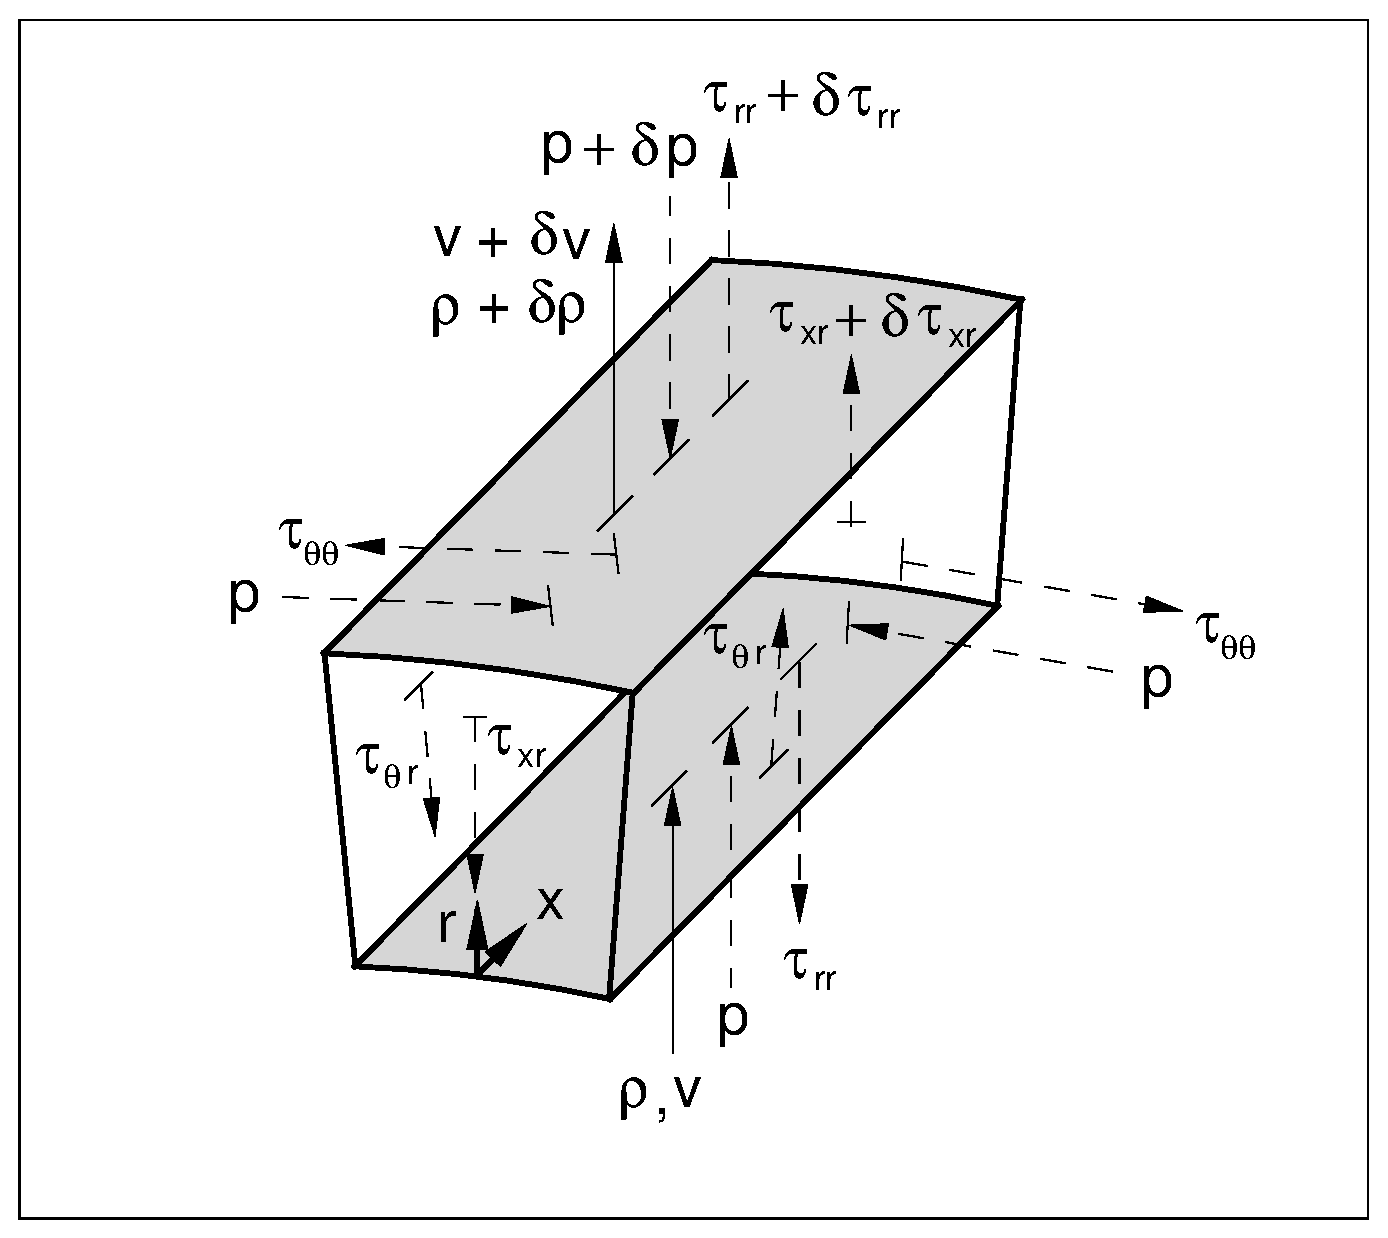
\includegraphics[height=5cm]{./rdir.eps}
% One can specify [angle=x,width=y,height=z] for the graphics
\caption[$x$ - $\theta$ planes]{$x$ - $\theta$ planes : All fluid properties are depicted by solid lines while 
				forces acting on the infantesimal fluid element are depicted by dashed lines (these include
				the pressure acting on the lower and upper $x$ - $\theta$ planes, as well as the left
				and right $x$ - $r$ planes and the shear acting on all faces of the volume)}
\label{fig:rdir}
\end{figure}

\begin{displaymath}
	\begin{array}{ccc}
		\begin{array}{c}
			\textrm{Mass flow of species \emph{k}} \\ \textrm{in through the bottom $x$ - $\theta$ plane} 
		\end{array} & 
	= & (\rho_k v)dx(R_o \theta) + j_{k_r} dx(R_o \theta)\\
	& \\ & \\
		\begin{array}{c}
			\textrm{Mass flow of species \emph{k}} \\ \textrm{out through the top $x$ - $\theta$ plane}
		\end{array} & 
	= & \begin{array}{c}
		(\rho_k + \frac{\partial \rho_k}{\partial r}dr)(v + \frac{\partial v}{\partial r}dr)dx
		(R_o + dr) \theta  \\
	+ (j_{k_r} + \frac{\partial j_{k_r}}{\partial r}dr)dx (R_o + dr) \theta
		\end{array}
	\end{array}
\end{displaymath}

	Taking the difference between the outflow and inflow in the $r$ direction yields,

\begin{displaymath}
	\begin{array}{ccc}
	\Delta \dot{m}_{k_r} & = &
		\begin{array}{c} 
	\Big\{(\rho_k v + j_{k_r} + \rho_k \frac{\partial v}{\partial r}dr + v \frac{\partial \rho_k}
	{\partial r}dr + \frac{\partial v}{\partial r} \frac{\partial \rho_k}{\partial r}dr^2 + \frac{\partial j_{k_r}}
	{\partial r}dr) -\rho_k v - j_{k_r}\Big\} dx(R_o \theta) \\
	+ (\rho_k v + j_{k_r} + \rho_k \frac{\partial v}{\partial r}dr + v \frac{\partial \rho_k}
	{\partial r}dr + \frac{\partial v}{\partial r} \frac{\partial \rho_k}{\partial r}dr^2 + \frac{\partial j_{k_r}}
	{\partial r}dr) dx dr \theta
		\end{array}
	\end{array}
\end{displaymath}

	Again combining differentials using the inverse of the chain rule and neglecting triple products (and higher)
of differentials, the above equation reduces to the following,

\begin{displaymath}
	\Delta \dot{m}_{k_r} = \Big( \frac{\partial \rho_k v}{\partial r} + \frac{\partial j_{k_r}}{\partial r}
	\Big)dxdr(R_o \theta) + (\rho_k v + j_{k_r})dxdr\theta
\end{displaymath}

	Applying the principle of mass conservation, any unsteady change in $\rho_k$ plus the sum of the mass fluxes in 
each of the co-ordinate directions must sum to zero,

\begin{displaymath}
	\begin{array}{ccc}
	\frac{\partial \rho_k}{\partial t}dxdr(R_o \theta) + \Delta \dot{m}_{k_x} + \Delta \dot{m}_{k_r} & = & 0 \\
	\Big\{(\frac{\partial \rho_k}{\partial t} + \frac{\partial \rho_k u}{\partial x} + \frac{\partial j_{k_x}}{\partial x}
	+  \frac{\partial \rho_k v}{\partial r} + \frac{\partial j_{k_r}}{\partial r})(R_o \theta) + 
	(\rho_k v + j_{k_r})\theta \Big\}dxdr & = & 0
	\end{array}
\end{displaymath}

	Without loss in generality, one can let $R_o \theta$ = 1 as shown in Fig. \ref{fig:inftes} and if one rewrites $R_o$ 
as $r$ then $\theta$ can be expressed as,	

\begin{equation}
	\theta = \frac {1}{r}
\label{eqn:theta}
\end{equation}

	which then allows the axisymmetric species conservation equation to be written as,

\begin{equation}
	\frac{\partial \rho_k}{\partial t} + \frac{\partial \rho_k u}{\partial x} + \frac{\partial \rho_k v}{\partial r}
	+ \frac {1}{r}(\rho_k v) = -\frac{\partial j_{k_x}}{\partial x} - \frac{\partial j_{k_r}}{\partial r} - \frac {1}{r}
	(j_{k_r})
\label{eqn:species}
\end{equation}

	For multi-species flow, the total density can be expressed as the sum of the individual species densities

\begin{equation}
	\sum_{i} \rho_k
\end{equation}

	while the concentration of species \emph{k}, $c_k$, can be written as 

\begin{equation}
	\rho_k = c_k \rho
\label{eqn:conc}
\end{equation}

	To express the diffusive flux in term of species concentrations one can use Fick's Law,

\begin{equation}
	j_{k_x} = - \rho D_{kl} \frac{\partial c_k}{\partial x}
\label{eqn:fick}
\end{equation}

	where $D_{kl}$ is the binary diffusion coefficient representing the degree to which gas $k$ will tend to 
diffuse into gas $l$ and the negative sign reflects the fact that the gas diffuses in the direction opposite the
concentration gradient (also note $j_{k_r}$ is similarly defined).  If we define another co-efficient $\nu_i$ as,

\begin{equation}
	\nu_k = \rho D_{kl}
\label{eqn:nuk}
\end{equation}

	then by substituting Eqs. \ref{eqn:fick} and \ref{eqn:nuk} into Eq. \ref{eqn:species} one obtains 

\begin{equation}
	\frac{\partial}{\partial t}(\rho_k) + \frac{\partial}{\partial x}(\rho_k u) + \frac{\partial}{\partial r}(\rho_k v)
	+ \frac {1}{r}(\rho_k v) = \frac{\partial}{\partial x}(\nu_k \frac{\partial c_k}{\partial x}) + \frac{\partial}
	{\partial r}(\nu_k \frac{\partial c_k}{\partial r}) + \frac {1}{r}(\nu_k \frac{\partial c_k}{\partial r})
\label{eqn:speciesfinal}
\end{equation}

	To obtain the global continuity equation, simply sum Eq.\ref{eqn:speciesfinal} over all the species present.
Since the sum of the species concentrations is unity ($\sum c_k = 1$), the sum of $\rho_k$ simplifies to $\rho$ 
(see Eq.\ref{eqn:conc} while any derivatives involving species concentrations reduce to zero yielding,

\begin{equation}
	\frac{\partial}{\partial t}(\rho) + \frac{\partial}{\partial x}(\rho u) + \frac{\partial}{\partial r}(\rho v)
	+ \frac{1}{r}(\rho v) = 0
\label{eqn:globalcont}
\end{equation}
	
%---------------------------------------------------------------------------------------------------------------------------
\subsection{Momentum Along the $x$ Co-Ordinate Direction}

	In order to derive the momentum equations in both the $x$ and $r$ directions, we will again make use of Figs.
\ref{fig:xdir} and \ref{fig:rdir}.  Since the desired equations are based on Newton's second law, ($F=ma$), the forces
acting on the surface of the infantesimal volume must be properly considered as it is these forces which balance the 
net change in momentum of the volume.  It should be noted at this point that given the axisymmetric assumption 
(Eq.\ref{eqn:dtheta}) no quantites passing through the $x$ - $r$ planes need be considered as there will be no net 
change in these quantites (i.e. the net change in $x$ momentum passing through these planes will be zero).  This 
also hold true for the $r$ co-ordinate direction.    

\begin{displaymath}
	\begin{array}{ccc}
		\textrm{$x$ Momentum in through the front $r$ - $\theta$ plane} &
		= & (\rho u)(u)dr(R_o \theta)\\
 		& \\ & \\
		\textrm{$x$ Momentum out through the back $r$ - $\theta$ plane} &
		= & (\rho u + \frac{\partial \rho u}{\partial x}dx)(u + \frac{\partial u}{\partial x}dx)dr(R_o \theta) 
	\end{array}
\end{displaymath}

	Taking the difference between the outflow and inflow $r$ - $\theta$ planes yields,

\begin{displaymath}
	\begin{array}{c}
	\Delta x_{momentum_{r \theta}}=(\rho u^2 + \rho u \frac{\partial u}{\partial x}dx + 
	u \frac{\partial \rho u}{\partial x}dx +
	\frac{\partial\rho u}{\partial x} \frac{\partial u}{\partial x}dx^2 - \rho u^2)dr(R_o \theta) \\ \\
	\Delta x_{momentum_{r \theta}}=(\frac{\partial \rho u^2}{\partial x})dxdr(R_o \theta)
	\end{array}
\end{displaymath}

	after combining derivatives and neglecting triple products of differentials.

\begin{displaymath}
	\begin{array}{ccc}
		\textrm{$x$ Momentum in through the bottom $x$ - $\theta$ plane} &
		= & (\rho v)(u)dx(R_o \theta)\\
 		& \\ & \\
		\textrm{$x$ Momentum out through the top $x$ - $\theta$ plane} &
		= & (\rho v + \frac{\partial \rho v}{\partial r}dr)(u + \frac{\partial u}{\partial r}dr)dx
		(R_o + dr) \theta 
	\end{array}
\end{displaymath}

	Taking the difference between the outflow and inflow $x$ - $\theta$ planes yields,

\begin{displaymath}
	\begin{array}{c}
	\Delta x_{momentum_{x \theta}}=
		\begin{array}{c}
	(\rho uv + \rho v \frac{\partial u}{\partial r}dr + 
	u \frac{\partial \rho v}{\partial r}dr + \frac{\partial u}{\partial r} \frac{\partial \rho v}{\partial r}dr^2 -
	\rho uv)dx(R_o \theta) \\
	 + (\rho uv + \rho v \frac{\partial u}{\partial r}dr + u \frac{\partial \rho v}{\partial r}dr + 
	\frac{\partial u}{\partial r} \frac{\partial \rho v}{\partial r}dr^2)dxdr \theta
		\end{array} \\ \\
	\Delta x_{momentum_{x \theta}}= (\frac{\partial \rho uv}{\partial r})dxdr (R_o \theta) + (\rho uv)dxdr \theta
	\end{array}
\end{displaymath}

	after again simplifying and neglecting triple products and higher of differential quantities.  Allowing for an
unsteady change in the $x$ direction momentum and applying Newton's second law yields,

\begin{displaymath}
	\frac{\partial \rho u}{\partial t}dxdr(R_o \theta) + \Delta x_{momentum_{r \theta}} + \Delta x_{momentum_{x \theta}} = 
	\sum \textrm{Forces}_x
\end{displaymath}

	which after making the appropriate substitutions yields

\begin{displaymath}
	\Big\{(\frac{\partial \rho u}{\partial t} + \frac{\partial \rho u^2}{\partial x} +
	\frac{\partial \rho uv}{\partial r})(R_o \theta) + (\rho u v) \theta\Big\}dxdr = \sum \textrm{Forces}_x
\end{displaymath}

	However, $\theta$ can be eliminated through the use of Eq. \ref{eqn:theta} to obtain

\begin{equation}
	\Big\{\frac{\partial \rho u}{\partial t} + \frac{\partial \rho u^2}{\partial x} +
	\frac{\partial \rho uv}{\partial r} + \frac{1}{r}(\rho u v)\Big\}dxdr = \sum \textrm{Forces}_x
\label{eqn:xmomchg}
\end{equation}

	To complete the right side of Eq.\ref{eqn:xmomchg}, one needs to consider the forces acting in the $x$ direction,
shown in Fig. \ref{fig:xdir} as dashed lines.
The forces that need to be considered are the pressure acting on the $r$ - $\theta$ planes 
(which always acts towards the interior of the volume), the tangential shear acting on the $x$ - $r$ and $x$ - $\theta$ 
planes ($\tau_{\theta x}$ and $\tau_{rx}$ respectively),
and the normal shear acting as well on the $r$ - $\theta$ planes (which always acts away from the interior
of the volume).  Also note that if turbulence is being considered then the pressure is the sum of the thermodynamic
pressure (as defined by some appropriate equation of state) and the turbulent pressure (which depends on the kinetic
energy of turbulence, $\rho k$)

\begin{displaymath}
	p = p_{thermodynamic} + \frac{2}{3}\rho k
\end{displaymath}

\begin{displaymath}
	\begin{array}{ccc}
		\begin{array}{c}
		\textrm{Force exerted on the front $r$ - $\theta$ plane} \\
		\textrm{by the pressure on its surface}
		\end{array} & = &
		p dr (R_o \theta) \\
	& \\ & \\
		\begin{array}{c}
		\textrm{Force exerted on the back $r$ - $\theta$ plane}\\
		\textrm{by the pressure on its surface}
		\end{array} & = &
		-(p + \frac{\partial p}{\partial x}dx) dr (R_o \theta) 
	\end{array} 
\end{displaymath}
\\
\begin{displaymath}
	\begin{array}{ccc}
		\begin{array}{c}
		\textrm{Force exerted on the front $r$- $\theta$ plane} \\
		\textrm{by the shear on its surface}
		\end{array} & = &
		- \tau_{xx}dr (R_o \theta) \\
   	& \\ & \\
		\begin{array}{c}
		\textrm{Force exerted on the back $r$ - $\theta$ plane}\\
		\textrm{by the shear on its surface}
		\end{array} & = &
		(\tau_{xx} + \frac{\partial \tau_{xx}}{\partial x}dx) dr (R_o \theta) 
	\end{array}
\end{displaymath}
\\
\begin{displaymath}
	\begin{array}{ccc}
		\begin{array}{c}
		\textrm{Force exerted on the bottom $x$ - $\theta$ plane}\\
		\textrm{by the shear on its surface}
		\end{array} & = &
		- \tau_{rx}dx(R_o \theta) \\
	& \\ & \\
		\begin{array}{c}
		\textrm{Force exerted on the top $x$ - $\theta$ plane} \\
		\textrm{by the shear on its surface}
		\end{array} & = &
		(\tau_{rx} + \frac{\partial \tau_{rx}}{\partial r}dr)dx(R_o + dr)\theta
	\end{array} 
\end{displaymath}

	Note that since the remaining shear acting in the $x$ direction, $\tau_{\theta x}$, is independent of the $x$ - $r$
plane upon which it acts due to the condition expressed in Eq. \ref{eqn:dtheta}, by inspection one can see that the forces
created by these shears will exactly cancel out in the $x$ direction.  However, summing the remaining terms yields,

\begin{displaymath}
	\begin{array}{ccc}
	\sum \textrm{Forces}_x & = &
		\begin{array}{c}
			(pdr - pdr - \frac{\partial p}{\partial x}dxdr - \tau_{xx}dr + \tau_{xx}dr + \frac{\partial \tau_{xx}}
			{\partial x}dxdr \\
			- \tau_{rx}dx + \tau_{rx}dx + \frac{\partial \tau_{rx}}{\partial r}dxdr)(R_o \theta)
			+ (\tau_{rx} + \frac{\partial \tau_{rx}}{\partial r}dr)dxdr \theta
		\end{array}
	\end{array}
\end{displaymath}

	which after canceling like terms, inserting Eq. \ref{eqn:theta} to replace $\theta$, and neglecting 
triple products of differentials reduces to

\begin{equation}
	\begin{array}{ccc}
	\sum \textrm{Forces}_x & = &
		(- \frac{\partial p}{\partial x} + \frac{\partial \tau_{xx}}{\partial x}
		+ \frac{\partial \tau_{rx}}{\partial r} + \frac{1}{r}\tau_{rx})dxdr
	\end{array}
\label{eqn:xforces}
\end{equation}

	Combining Eqs. \ref{eqn:xmomchg} and \ref{eqn:xforces} one obtains

\begin{equation}
\Big\{\frac{\partial}{\partial t}(\rho u) + \frac{\partial}{\partial x}(\rho u^2) +
\frac{\partial}{\partial r}(\rho uv) + \frac{1}{r}(\rho u v)\Big\}dxdr = \Big\{ - \frac{\partial}{\partial x}(p) 
+ \frac{\partial}{\partial x}(\tau_{xx}) + \frac{\partial}{\partial r}(\tau_{rx}) + \frac{1}{r}(\tau_{rx})\Big\}dxdr
\label{eqn:xmomshear}
\end{equation}

\subsubsection{Definition of the Viscous Stresses}

	From the mechanics of Newtonian fluids the stresses can be defined using derivatives of the 
co-ordinate velocities as follows

\begin{equation}
	\tau_{rx} = \tau_{xr} = \mu(\frac{\partial v}{\partial x} + \frac{\partial u}{\partial r})
\label{eqn:taurx}
\end{equation}

\begin{equation}
	\tau_{xx} = \lambda(\nabla \cdot \vec{V}) + 2 \mu \frac{\partial u}{\partial x}
\label{eqn:tauxxlambda}
\end{equation}

\begin{equation}
	\tau_{rr} = \lambda(\nabla \cdot \vec{V}) + 2 \mu \frac{\partial v}{\partial r}
\label{eqn:taurrlambda}
\end{equation}

\begin{displaymath}
	\tau_{\theta \theta} = \lambda(\nabla \cdot \vec{V}) + 2 \mu (\frac{1}{r} \frac{\partial w}{\partial \theta} + \frac{v}{r})
\end{displaymath}

	which for the axisymmetric case (Eq. \ref{eqn:dtheta}) reduces to 

\begin{equation}
	\tau_{\theta \theta} = \lambda(\nabla \cdot \vec{V}) + 2 \mu \frac{v}{r}	
\label{eqn:tauthetathetalambda}
\end{equation}
	
	The quantity $\vec{V}$ is the vector sum of the co-ordinate velocties and $\mu$ is the coefficient of 
viscosity of the fluid under consideration.  In order to evaluate the dot product of the del operator ($\nabla$) on 
the velocity vector ($\vec{V}$) one must remember to use the cylindrical co-ordinate system,

\begin{displaymath}
	\nabla \cdot \vec{V} = \frac{\partial u}{\partial x} + \frac{1}{r} \frac{\partial rv}{\partial r} + \frac{1}{r}
	\frac{\partial w}{\partial \theta}
\end{displaymath}

	which after applying the axisymmetric condition (Eq. \ref{eqn:dtheta}) and the chain rule from the Calculus
can be reduced to

\begin{equation}
	\nabla \cdot \vec{V} = \frac{\partial u}{\partial x} +  \frac{\partial v}{\partial r} + \frac{v}{r}
\label{eqn:delv}
\end{equation}

	With the help of Stokes' hypothesis which states

\begin{equation}
	\lambda = -\frac{2}{3} \mu
\label{eqn:stokes}
\end{equation}

	one can rewrite the stress quantities in terms of velocity component derivatives by substituting Eqs. \ref{eqn:delv} and
\ref{eqn:stokes} into Eqs. \ref{eqn:tauxxlambda} - \ref{eqn:tauthetathetalambda},

\begin{displaymath}
	\tau_{xx} = - \frac{2}{3} \mu (\frac{\partial u}{\partial x} + \frac{\partial v}{\partial r} + \frac{v}{r}) 
	+ \frac{6}{3} \mu \frac{\partial u}{\partial x}
\end{displaymath}

\begin{displaymath}
	\tau_{xx} = \mu ( \frac{4}{3} \frac{\partial u}{\partial x} - \frac{2}{3} \frac{\partial v}{\partial r})  
	- \mu \frac{2}{3} \frac{v}{r} 
\end{displaymath}

\begin{displaymath}
	\tau_{rr} = - \frac{2}{3} \mu (\frac{\partial u}{\partial x} + \frac{\partial v}{\partial r} + \frac{v}{r}) 
	+ \frac{6}{3} \mu \frac{\partial v}{\partial x}
\end{displaymath}

\begin{displaymath}
	\tau_{rr} = \mu ( - \frac{2}{3} \frac{\partial u}{\partial x} + \frac{4}{3} \frac{\partial v}{\partial r})  
	- \mu \frac{2}{3} \frac{v}{r} 
\end{displaymath}

\begin{displaymath}
	\tau_{\theta \theta} = - \frac{2}{3} \mu (\frac{\partial u}{\partial x} + \frac{\partial v}{\partial r} 
	+ \frac{v}{r}) + \frac{6}{3}\mu \frac{v}{r}
\end{displaymath}

\begin{equation}
	\tau_{\theta \theta} = \mu \Big\{- \frac{2}{3} (\frac{\partial u}{\partial x} + \frac{\partial v}{\partial r})  
	+ \frac{4}{3} \frac{v}{r} \Big\} 
\label{eqn:tauthetatheta}
\end{equation}

	If we further define $\hat{\tau}_{xx}$ and $\hat{\tau}_{rr}$ to be 

\begin{equation}
	\hat{\tau}_{xx} =  \mu ( \frac{4}{3} \frac{\partial u}{\partial x} - \frac{2}{3} \frac{\partial v}{\partial r})  
\label{eqn:tauxxhat}
\end{equation}

\begin{equation}
	\hat{\tau}_{rr} =  \mu ( - \frac{2}{3} \frac{\partial u}{\partial x} + \frac{4}{3} \frac{\partial v}{\partial r})  
\label{eqn:taurrhat}
\end{equation}

	then

\begin{equation}
	\tau_{xx} = \hat{\tau}_{xx} - \mu \frac{2}{3} \frac {v}{r}
\label{eqn:tauxx}
\end{equation}

\begin{equation}
	\tau_{rr} = \hat{\tau}_{rr} - \mu \frac{2}{3} \frac{v}{r}
\label{eqn:taurr}
\end{equation}

	This step of defining $\hat{\tau}$ is done so that all differences between the axisymmetric and more
conventional 2D equations can be kept to a single source term, since $\hat{\tau}$ now matches exactly the stresses
found from a 2D Cartesian derivation.
	
	Finally, by using the results of Eq. \ref{eqn:tauxx} in Eq. \ref{eqn:xmomshear} and 
rearranging leaving only viscosity related terms on the right side of the equation, one obtains the 
desired form of the $x$ direction momentum equation

\begin{equation}
\frac{\partial}{\partial t}(\rho u) + \frac{\partial}{\partial x}(\rho u^2 + p) +
\frac{\partial}{\partial r}(\rho uv) + \frac{1}{r}(\rho u v) = 
\frac{\partial}{\partial x}(\hat{\tau}_{xx}) + \frac{\partial}{\partial r}(\tau_{rx}) + 
\frac{1}{r}(\tau_{rx}) - \frac{2}{3} \frac{\partial}{\partial x}(\mu \frac{v}{r})
\label{eqn:xmom}
\end{equation}

	with the stresses defined by their respective Eqs.\ref{eqn:taurx} and \ref{eqn:tauxxhat}.

%---------------------------------------------------------------------------------------------------------------------------
\subsection{Momentum Along the $r$ Co-Ordinate Direction}

	To obtain this equation, one needs to consider the quantities shown in Fig. \ref{fig:rdir}.  The derivation of 
this equation is similar to that of the $x$ direction but for a few extra terms acting in the $\theta$ direction that need 
be considered due to their influence in the $r$ direction.

\begin{displaymath}
	\begin{array}{ccc}
		\textrm{$r$ Momentum in through the bottom $x$ - $\theta$ plane} &
		= & (\rho v)(v)dx(R_o \theta)\\
 		& \\ & \\
		\textrm{$r$ Momentum out through the top $x$ - $\theta$ plane} &
		= & (\rho v + \frac{\partial \rho v}{\partial r}dr)(v + \frac{\partial v}{\partial r}dr)dx
		(R_o + dr) \theta 
	\end{array}
\end{displaymath}


	Taking the difference between the outflow and inflow $x$ - $\theta$ planes yields,

\begin{displaymath}
	\begin{array}{c}
	\Delta r_{momentum_{x \theta}}=
		\begin{array}{c}
	(\rho v^2 + \rho v \frac{\partial v}{\partial r}dr + 
	v \frac{\partial \rho v}{\partial r}dr + \frac{\partial v}{\partial r} \frac{\partial \rho v}{\partial r}dr^2 -
	\rho v^2)dx(R_o \theta) \\
	 + (\rho v^2 + \rho v \frac{\partial v}{\partial r}dr + v \frac{\partial \rho v}{\partial r}dr + 
	\frac{\partial v}{\partial r} \frac{\partial \rho v}{\partial r}dr^2)dxdr \theta
		\end{array} \\ \\
	\Delta r_{momentum_{x \theta}}= (\frac{\partial \rho v^2}{\partial r})dxdr (R_o \theta) + (\rho v^2)dxdr \theta
	\end{array}
\end{displaymath}

\begin{displaymath}
	\begin{array}{ccc}
		\textrm{$r$ Momentum in through the front $r$ - $\theta$ plane} &
		= & (\rho v)(u)dr(R_o \theta)\\
 		& \\ & \\
		\textrm{$r$ Momentum out through the back $r$ - $\theta$ plane} &
		= & (\rho v + \frac{\partial \rho v}{\partial x}dx)(u + \frac{\partial u}{\partial x}dx)dr(R_o \theta) 
	\end{array}
\end{displaymath}

	Taking the difference between the outflow and inflow $r$ - $\theta$ planes yields,

\begin{displaymath}
	\begin{array}{c}
	\Delta r_{momentum_{r \theta}}=(\rho uv + \rho v \frac{\partial u}{\partial x}dx + 
	u \frac{\partial \rho v}{\partial x}dx +
	 \frac{\partial u}{\partial x} \frac{\partial\rho v}{\partial x}dx^2 - \rho uv)dr(R_o \theta) \\ \\
	\Delta r_{momentum_{r \theta}}=(\frac{\partial \rho uv}{\partial x})dxdr(R_o \theta)
	\end{array}
\end{displaymath}

	As before, allowing for an unsteady change in the $r$ direction momentum and applying Newton's second law

\begin{displaymath}
	\frac{\partial \rho v}{\partial t}dxdr(R_o \theta) + \Delta r_{momentum_{r \theta}} + \Delta r_{momentum_{x \theta}} = 
	\sum \textrm{Forces}_r
\end{displaymath}

	which after making the appropriate substitutions yields

\begin{displaymath}
	\Big\{(\frac{\partial \rho v}{\partial t} + \frac{\partial \rho uv}{\partial x} +
	\frac{\partial \rho v^2}{\partial r})(R_o \theta) + (\rho v^2 \theta)\Big\}dxdr = \sum \textrm{Forces}_r
\end{displaymath}

	However, $\theta$ can be eliminated through the use of Eq. \ref{eqn:theta} to obtain

\begin{equation}
	\Big\{\frac{\partial \rho v}{\partial t} + \frac{\partial \rho uv}{\partial x} +
	\frac{\partial \rho v^2}{\partial r} + \frac{1}{r}(\rho v^2)\Big\}dxdr = \sum \textrm{Forces}_r
\label{eqn:rmomchg}
\end{equation}

	Again examining each of the forces contributing to an overall force in the $r$ direction individually one 
can complete the right hand side of Eq.\ref{eqn:rmomchg}.

\begin{displaymath}
	\begin{array}{ccc}
		\begin{array}{c}
		\textrm{Force exerted on the bottom $x$ - $\theta$ plane} \\
		\textrm{by the pressure on its surface}
		\end{array} & = &
		p dx (R_o \theta) \\
	& \\ & \\
		\begin{array}{c}
		\textrm{Force exerted on the top $x$ - $\theta$ plane}\\
		\textrm{by the pressure on its surface}
		\end{array} & = &
		-(p + \frac{\partial p}{\partial r}dr) dx (R_o + dr) \theta
	\end{array} 
\end{displaymath}
\\
\begin{displaymath}
	\begin{array}{ccc}
		\begin{array}{c}
		\textrm{Force exerted on the bottom $x$- $\theta$ plane} \\
		\textrm{by the shear on its surface}
		\end{array} & = &
		- \tau_{rr}dx (R_o \theta) \\
   	& \\ & \\
		\begin{array}{c}
		\textrm{Force exerted on the top $x$ - $\theta$ plane}\\
		\textrm{by the shear on its surface}
		\end{array} & = &
		(\tau_{rr} + \frac{\partial \tau_{rr}}{\partial r}dr) dx (R_o + dr) \theta
	\end{array}
\end{displaymath}

\begin{displaymath}
	\begin{array}{ccc}
		\begin{array}{c}
		\textrm{Force exerted on the front $r$- $\theta$ plane} \\
		\textrm{by the shear on its surface}
		\end{array} & = &
		- \tau_{xr}dr (R_o \theta) \\
   	& \\ & \\
		\begin{array}{c}
		\textrm{Force exerted on the back $r$ - $\theta$ plane}\\
		\textrm{by the shear on its surface}
		\end{array} & = &
		(\tau_{xr} + \frac{\partial \tau_{xr}}{\partial x}dx) dr (R_o \theta) 
	\end{array}
\end{displaymath}

	Now, by symmetry, it can be see that since $\tau_{\theta r}$ acts in opposite directions and on opposite
faces of the fluid element, it's net effect in the $r$ direction will be zero due to the axisymmetric condtion
expressed by Eq.\ref{eqn:dtheta}.  This can be illustrated by the following.  If one places the $x$ - $r$ plane
at the centre of the infantesimal volume, then the distance to each boundary $x$ - $r$ plane (the left and right sides
of the volume) is $\frac{\theta}{2}$.  The component of $\tau_{\theta r}$ acting on each of these faces in the $r$ 
direction is $\tau_{\theta r}\cos{\frac{\theta}{2}}$.  Therefore, given that the direction each of these components 
acts is opposed, their overall contribution to the right hand side of Eq.\ref{eqn:rmomchg} is zero.  However, the same 
cannot be said for $\tau_{\theta \theta}$, and indeed $p$, which also 
acts on these surfaces.  In these cases, there is a net effect which must be accounted for as follows.

\begin{displaymath}
	\begin{array}{ccc}
		\begin{array}{c}
		\textrm{Force exerted on the left $x$- $r$ plane} \\
		\textrm{in the $r$ direction} \\
		\textrm{by the shear on its surface}
		\end{array} & = &
		- \tau_{\theta \theta}\sin{\frac{\theta}{2}}dxdr \\
   	& \\ & \\
		\begin{array}{c}
		\textrm{Force exerted on the right $x$ - $r$ plane}\\
		\textrm{in the $r$ direction} \\
		\textrm{by the shear on its surface}
		\end{array} & = &
		- \tau_{\theta \theta}\sin{\frac{\theta}{2}}dxdr
	\end{array}
\end{displaymath}  

\begin{displaymath}
	\begin{array}{ccc}
		\begin{array}{c}
		\textrm{Force exerted on the left $x$- $r$ plane} \\
		\textrm{in the $r$ direction} \\
		\textrm{by the pressure on its surface}
		\end{array} & = &
		p \sin{\frac{\theta}{2}}dxdr \\
   	& \\ & \\
		\begin{array}{c}
		\textrm{Force exerted on the right $x$ - $r$ plane}\\
		\textrm{in the $r$ direction} \\
		\textrm{by the pressre on its surface}
		\end{array} & = &
		p \sin{\frac{\theta}{2}}dxdr
	\end{array}
\end{displaymath}  

	but for small angles (as is the case for an infantesimal volume),

\begin{equation}
	\sin{\theta} = \theta
\label{eqn:smallangle}
\end{equation}

	therefore,

\begin{displaymath}
	\begin{array}{ccc}
		\begin{array}{c}
		\textrm{Force exerted on the left $x$- $r$ plane} \\
		\textrm{in the $r$ direction} \\
		\textrm{by the shear on its surface}
		\end{array} & = &
		- \frac{1}{2}\tau_{\theta \theta}\theta dxdr \\
   	& \\ & \\
		\begin{array}{c}
		\textrm{Force exerted on the right $x$ - $r$ plane}\\
		\textrm{in the $r$ direction} \\
		\textrm{by the shear on its surface}
		\end{array} & = &
		- \frac{1}{2} \tau_{\theta \theta}\theta dxdr
	\end{array}
\end{displaymath}

\begin{displaymath}
	\begin{array}{ccc}
		\begin{array}{c}
		\textrm{Force exerted on the left $x$- $r$ plane} \\
		\textrm{in the $r$ direction} \\
		\textrm{by the pressure on its surface}
		\end{array} & = &
		\frac{1}{2}p \theta dxdr \\
   	& \\ & \\
		\begin{array}{c}
		\textrm{Force exerted on the right $x$ - $r$ plane}\\
		\textrm{in the $r$ direction} \\
		\textrm{by the pressure on its surface}
		\end{array} & = &
		\frac{1}{2}p \theta dxdr
	\end{array}
\end{displaymath}

	Summing all the forces considered, the total force in the $r$ - direction yields,

\begin{displaymath}
	\begin{array}{ccc}
	\sum \textrm{Forces}_r & = &
		\begin{array}{c}
			(pdx - pdx  - \frac{\partial p}{\partial r}dxdr - \tau_{rr}dx + \tau_{rr}dx + 
			\frac{\partial \tau_{rr}}{\partial r}dxdr - \tau_{xr}dr + \tau_{xr}dr 
			 + \frac{\partial \tau_{xr}}{\partial x} dxdr)
			(R_o \theta) \\
			+ (-p -\frac{\partial p}{\partial r}dr + \tau_{rr} + \frac{\partial \tau_{rr}}{\partial r}dr
			+ \frac{1}{2}p + \frac{1}{2}p - \frac{1}{2}\tau_{\theta \theta} \theta 
			- \frac{1}{2}\tau_{\theta \theta}) dxdr\theta
		\end{array}
	\end{array}
\end{displaymath}

	which after cancelling like terms, inserting Eq. \ref{eqn:theta} to replace $\theta$, and neglecting 
triple products of differentials reduces to

\begin{equation}
	\begin{array}{ccc}
	\sum \textrm{Forces}_r & = &
		\Big\{- \frac{\partial p}{\partial r} + \frac{\partial \tau_{xr}}{\partial x}
		+ \frac{\partial \tau_{rr}}{\partial r} + \frac{1}{r}(\tau_{rr} - \tau_{\theta \theta})\Big\}dxdr
	\end{array}
\label{eqn:rforces}
\end{equation}

	As before, substituting Eq.\ref{eqn:taurr} into Eq.\ref{eqn:rforces} for $\tau_{rr}$ and combining
the result with Eq.\ref{eqn:rmomchg} (leaving only viscous terms on the right hand side) yields the desired form
of the $r$ momentum equation,

\begin{equation}
\frac{\partial}{\partial t}(\rho v) + \frac{\partial}{\partial x}(\rho uv) +
\frac{\partial}{\partial r}(\rho v^2 + p) + \frac{1}{r}(\rho v^2) = 
\frac{\partial}{\partial x}(\tau_{xr}) + \frac{\partial}{\partial r}(\hat{\tau}_{rr}) + 
\frac{1}{r}(\hat{\tau}_{rr} - \tau_{\theta \theta} - \frac{2}{3} \mu \frac{v}{r})
- \frac{2}{3} \frac{\partial}{\partial r}(\mu \frac{v}{r})
\label{eqn:rmom}
\end{equation}

	with the stresses defined by their respective Eqs.\ref{eqn:taurx},\ref{eqn:tauthetatheta}, and \ref{eqn:taurrhat}.

%--------------------------------------------------------------------------------------------------------------------------
\subsection{Energy Equation}

	To derive the complete energy equation for a multi-species, viscous, turbulent, axisymmetric flow, it is helpful to 
consider each source of energy transfer across the infantesimal volume boundaries individually.  In general, the 
complete energy equation can be expressed as follows

\begin{displaymath}
	\begin{array}{ccc}
		\begin{array}{c}
		\textrm{Rate of Change} \\ \textrm{of Total} \\ \textrm{Energy Inside} \\ \textrm{Infantesimal Volume}
		\end{array} & = &
	   \begin{array}{ccc}
		\begin{array}{c}
		\textrm{Energy Transfer} \\ \textrm{into Infantesimal}\\ \textrm{Volume due to}\\ \textrm{Species Diffusion}
		\end{array} & + &
		\begin{array}{c}
		\textrm{Energy Transfer} \\ \textrm{into Infantesimal}\\ \textrm{Volume due to Heat}
		\end{array}  
		\\ & + & \\
		\begin{array}{c}
		\textrm{Rate of Work}\\ \textrm{Done on} \\ \textrm{Infantesimal Volume}
		\end{array} & + &
		\begin{array}{c}
		\textrm{Energy Transfer} \\ \textrm{into Infantesimal}\\ \textrm{Volume due to}\\ 
		\textrm{Turbulence Diffusion}  
		\end{array}
	   \end{array}
	\end{array}
\end{displaymath}

\subsubsection{Rate of Change of Total Energy}

\begin{figure}[ht]
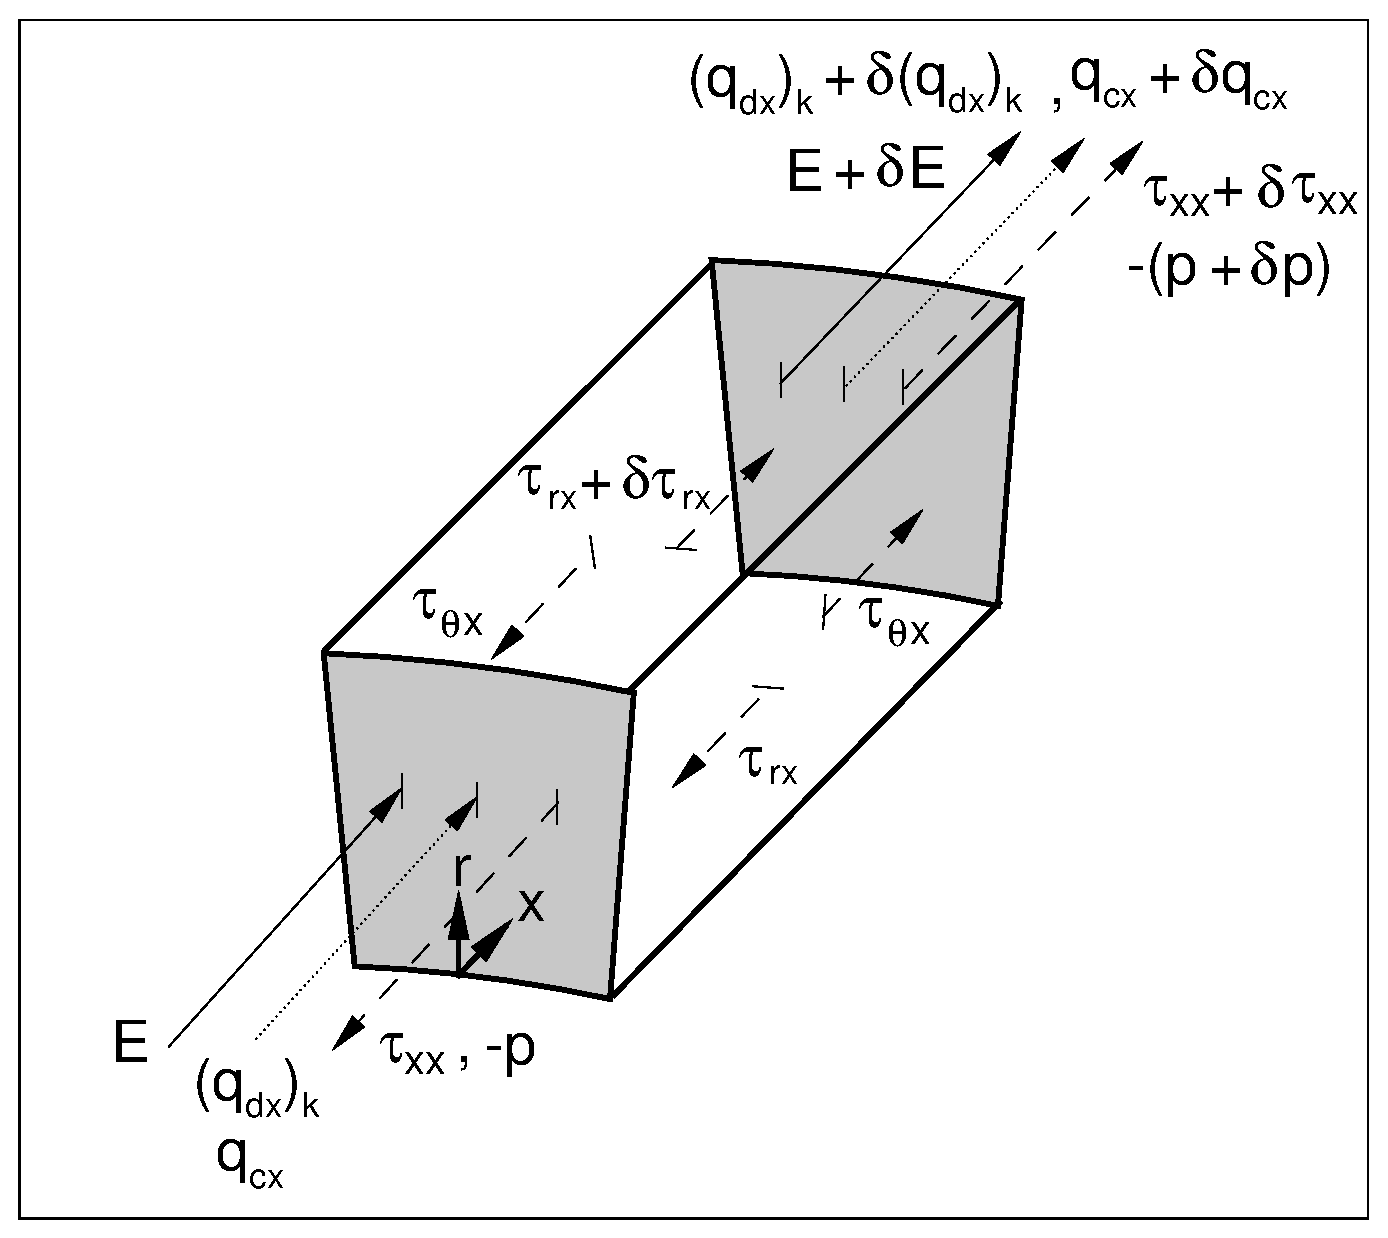
\includegraphics[height=5cm]{./xdirener.eps}
% One can specify [angle=x,width=y,height=z] for the graphics
\caption[$r$ - $\theta$ planes]{$r$ - $\theta$ planes : Energy itself is depicted by a solid line, forces  
				acting on the infantesimal fluid element are depicted by dashed lines (these
				are the same forces as in Fig. \ref{fig:xdir}) and the sources of energy
				transfer are depicted by dotted lines)}
\label{fig:xdirener}
\end{figure}

	For a infantesimal fluid volume in motion, the total energy is composed of internal energy, $\rho e$,
(where $e$ is the specific internal energy) and the kinetic energy due to motion $\frac{1}{2}\rho\vec{V}^2$.  
If $E$ represents the total \emph{specific} energy then

\begin{equation}
	E = e + \frac{1}{2}\vec{V}^2 
\label{eqn:spenergy}
\end{equation}

	From Fig. \ref{fig:xdirener} one can write

\begin{displaymath}
	\begin{array}{ccc}
		\textrm{Total Energy in the front $r$ - $\theta$ plane} & = & 
		(\rho E)u dr(R_o \theta) \\ & & \\
		\textrm{Total Energy out the back $r$ - $\theta$ plane} & = &
		(\rho E + \frac{\partial \rho E}{\partial x}dx)(u + \frac{\partial u}{\partial x}dx)dr(R_o \theta)
	\end{array}
\end{displaymath}	

	and from Fig. \ref{fig:rdirener}

\begin{displaymath}
	\begin{array}{ccc}
		\textrm{Total Energy in the bottom $x$ - $\theta$ plane} & = & 
		(\rho E)v dx(R_o \theta) \\ & & \\
		\textrm{Total Energy out the top $x$ - $\theta$ plane} & = &
		(\rho E + \frac{\partial \rho E}{\partial r}dr)(v + \frac{\partial v}{\partial r}dr)dx(R_o + dr)\theta
	\end{array}
\end{displaymath}

	Taking the net difference between the outflow and inflow and allowing for an unsteady change in the total energy
yields,

\begin{displaymath}
	\begin{array}{ccc}
		\begin{array}{c}
		\textrm{Rate of Change} \\ \textrm{of Total} \\ \textrm{Energy Inside} \\ \textrm{Infantesimal Volume}
		\end{array} & = &
		\begin{array}{c}
		(\rho E u dr + \rho E \frac{\partial u}{\partial x}dxdr + u \frac{\partial \rho E}{\partial x}dxdr +
		\frac{\partial u}{\partial x} \frac{\partial \rho E}{\partial x}dx^2dr - \rho E u dr + \rho E v dx \\
		+ \rho E \frac{\partial v}{\partial r}dxdr + v \frac{\partial \rho E}{\partial r}dxdr +
		\frac{\partial v}{\partial r} \frac{\partial \rho E}{\partial r}dxdr^2 - \rho E v dx  + \frac{\partial \rho E}
		{\partial t}dxdr)(R_o \theta) \\
		(\rho E v + \rho E \frac{\partial v}{\partial r}dr + v \frac{\partial \rho E}{\partial r}dr +
		\frac{\partial \rho E}{\partial r}\frac{\partial v}{\partial r}dr^2)dxdr \theta
		\end{array}
	\end{array}
\end{displaymath}

	After cancelling like terms and neglecting triple products and higher of differentials the above simplifies to

\begin{displaymath}
	\begin{array}{ccc}
		\begin{array}{c}
		\textrm{Rate of Change of Total Energy} \\ \textrm{Inside Infantesimal Volume}
		\end{array} & = &
		\Big\{( \frac{\partial \rho E}{\partial t} +\frac{\partial \rho E u}{\partial x} + \frac{\partial \rho E v}
		{\partial r})(R_o \theta) + (\rho E v)\theta \Big\}dxdr
	\end{array}
\end{displaymath}

	which after eliminating $\theta$ using Eq.\ref{eqn:theta} yields

\begin{equation}
	\begin{array}{ccc}
		\begin{array}{c}
		\textrm{Rate of Change of Total Energy} \\ \textrm{Inside Infantesimal Volume}
		\end{array} & = &
		\Big\{\frac{\partial \rho E}{\partial t} +\frac{\partial \rho E u}{\partial x} + \frac{\partial \rho E v}
		{\partial r} + \frac{1}{r}(\rho E v)\Big\}dxdr
	\end{array}
\label{eqn:energychange}
\end{equation}

\begin{figure}[hb]
\includegraphics[height=5cm]{./rdirener.eps}
% One can specify [angle=x,width=y,height=z] for the graphics
\caption[$r$ - $\theta$ planes]{$r$ - $\theta$ planes : Energy itself is depicted by a solid line, forces  
				acting on the infantesimal fluid element are depicted by dashed lines (these
				are the same forces as in Fig. \ref{fig:rdir}) and the sources of energy
				transfer are depicted by dotted lines)}
\label{fig:rdirener}
\end{figure}

\subsubsection{Energy Transfer due to Species Diffusion}

	Considering first species diffusion, from Eq.\ref{eqn:fick} one already has an expression for the rate
at which species diffusion occurs (as the units of the diffusive flux, $j_{k_x}$, are $kg/m^2 s$).  Hence to calculate the 
energy transfer occuring due to this flux, one needs only a quantity for the energy of the given species \emph{k}
per unit mass of species \emph{k}.  The specific enthalpy of a given species \emph{k}, $h_k$, has units of
$J/kg$ and is thus a suitable quanitity for determining the energy transfer due to species diffusion.  Therefore,

\begin{displaymath}
	\begin{array}{ccccc}
		\begin{array}{c}
			\textrm{Energy transfer due to species}\\ \textrm{diffusion in the $x$ direction}
		\end{array} 
		& = & (q_{d_x})_k & = & j_{k_x}h_k
		\\ & & & & \\
		\begin{array}{c}
			\textrm{Energy transfer due to species}\\ \textrm{diffusion in the $r$ direction} 
		\end{array}
		& = & (q_{d_r})_k & = & j_{k_r}h_k
	\end{array}
\end{displaymath} 

	which after substituting the results of Eqs. \ref{eqn:fick} and \ref{eqn:nuk} yields,

\begin{equation}
	(q_{d_x})_k = -\nu_k \frac{\partial c_k}{\partial x}h_k
\label{eqn:qdx}
\end{equation}

\begin{equation}
	(q_{d_r})_k = -\nu_k \frac{\partial c_k}{\partial r}h_k
\label{eqn:qdr}
\end{equation}

	Now, considering this energy flow in the $x$ direction first, as shown in Fig. \ref{fig:xdirener}, and
remembering to sum the total energy transfer over all the species \emph{k} present in the flow

\begin{displaymath}
	\begin{array}{ccc}
		\textrm{Energy in the front $r$ - $\theta$ plane} & = & \sum_k (q_{d_x})_kdr(R_o \theta) 
		\\ & & \\
		\textrm{Energy out the back $r$ - $\theta$ plane} & = & -\Big\{\sum_k (q_{d_x})_k + 
		\frac{\partial \sum_k (q_{d_x})_k}{\partial x}dx\Big\}dr(R_o \theta)
	\end{array}
\end{displaymath}

	while in the $r$ direction,

\begin{displaymath}
	\begin{array}{ccc}
		\textrm{Energy in the bottom $x$ - $\theta$ plane} & = & \sum_k (q_{d_r})_kdx(R_o \theta) 
		\\ & & \\
		\textrm{Energy out the top $x$ - $\theta$ plane} & = & -\Big\{\sum_k (q_{d_r})_k + 
		\frac{\partial \sum_k (q_{d_r})_k}{\partial r}dr\Big\}dx(R_o + dr) \theta
	\end{array}
\end{displaymath}

	Taking the sum of these quantities yields,

\begin{displaymath}
	\begin{array}{ccc}
		\begin{array}{c}
		\textrm{Net Energy Transfer} \\ \textrm{due to Species Diffusion}
		\end{array} & = &
			\begin{array}{c}
		\Big\{\sum_k (q_{d_x})_kdr - \sum_k (q_{d_x})_kdr - \frac{\partial \sum_k (q_{d_x})_k}{\partial x}dxdr \\
		+  \sum_k (q_{d_r})_kdx - \sum_k (q_{d_r})_kdx - \frac{\partial \sum _k(q_{d_r})_k}{\partial r}dxdr\Big\}
		(R_o \theta)\\
		\Big\{-\sum_k (q_{d_r})_k - \frac{\partial \sum_k (q_{d_r})_k}{\partial r}dr\Big\}dxdr \theta
			\end{array}
	\end{array}
\end{displaymath}

	which after simplifying, substituting Eq.\ref{eqn:theta} and neglecting triple products of differentials reduces to

\begin{equation}
	\begin{array}{ccc}
	\begin{array}{c}
	\textrm{Net Energy Transfer} \\ \textrm{due to Species Diffusion}
	\end{array} & = &
		\begin{array}{c}
			\Big\{-\frac{\partial \sum_k (q_{d_x})_k}{\partial x} - \frac{\partial \sum_k (q_{d_r})_k}{\partial r}
			- \frac{1}{r} \sum_k (q_{d_r})_k \Big\}dxdr	
		\end{array}
	\end{array}
\label{eqn:diff}
\end{equation}

	Combining the results of Eqs.\ref{eqn:energychange} and \ref{eqn:diff} and substituting Eqs.\ref{eqn:qdx} and
\ref{eqn:qdr}

\begin{displaymath}
	\begin{array}{ccc}
		\Big\{\frac{\partial \rho E}{\partial t} +\frac{\partial \rho E u}{\partial x} + \frac{\partial \rho E v}
		{\partial r} + \frac{1}{r}(\rho E v)\Big\}dxdr & = &
		\begin{array}{c}
			\Big\{\frac{\partial \sum_k (\nu_k \frac{\partial c_k}{\partial x}h_k)}{\partial x} 
			+ \frac{\partial \sum_k (\nu_k \frac{\partial c_k}{\partial r}h_k)}{\partial r}
			+ \frac{1}{r} \sum_k (\nu_k \frac{\partial c_k}{\partial r}h_k) + \ldots \Big\}dxdr	
		\end{array} 
	\end{array}
\end{displaymath}

\subsubsection{Energy Transfer due to Heat}

	The transfer of energy by heat follows the same logic as the transfer of energy by diffusion, only the
heat fluxes, $(q_c)_x$ and $(q_c)_r$ are defined by

\begin{equation}
	q_{c_x} = -\kappa \frac{\partial T}{\partial x} 
\label{eqn:xheatflux}
\end{equation}

\begin{equation}
	q_{c_r} = -\kappa \frac{\partial T}{\partial r}
\label{eqn:rheatflux}
\end{equation}	

	whose units are $J/m^2 s$ and where $k$ is the coefficient of thermal conductivity for the fluid 
as a whole (which can be found using a suitable mixing rule over all the individual species).  Thus for the $x$
direction

\begin{displaymath}
	\begin{array}{ccc}
		\textrm{Energy in the front $r$ - $\theta$ plane} & = & q_{c_x}dr(R_o \theta) 
		\\ & & \\
		\textrm{Energy out the back $r$ - $\theta$ plane} & = & -(q_{c_x} + 
		\frac{\partial q_{c_x}}{\partial x}dx)dr(R_o \theta)
	\end{array}
\end{displaymath}

	while in the $r$ direction,

\begin{displaymath}
	\begin{array}{ccc}
		\textrm{Energy in the bottom $x$ - $\theta$ plane} & = & q_{c_r}dx(R_o \theta) 
		\\ & & \\
		\textrm{Energy out the top $x$ - $\theta$ plane} & = & -(q_{c_r} + \frac{\partial q_{c_r}}
		{\partial r}dr)dx(R_o + dr) \theta
	\end{array}
\end{displaymath}

	Taking the sum of these quantities yields,

\begin{displaymath}
	\begin{array}{ccc}
		\begin{array}{c}
		\textrm{Net Energy Transfer} \\ \textrm{due to Heat}
		\end{array} & = &
			\begin{array}{c}
		q_{c_x}dr - q_{c_x}dr - \frac{\partial q_{c_x}}{\partial x}dxdr \\
		+  q_{c_r}dx - q_{c_r}dx - \frac{\partial q_{c_r}}{\partial r}dxdr)(R_o \theta)
		\\
		\Big\{-q_{c_r} - \frac{\partial q_{c_r}}{\partial r}dr\Big\}dxdr \theta
			\end{array}
	\end{array}
\end{displaymath}

	which after simplifying, substituting Eq.\ref{eqn:theta} and neglecting triple products of differentials reduces to

\begin{equation}
	\begin{array}{ccc}
	\begin{array}{c}
	\textrm{Net Energy Transfer} \\ \textrm{due to Heat}
	\end{array} & = &
		\begin{array}{c}
			(- \frac{\partial q_{c_x}}{\partial x} - \frac{\partial q_{c_r}}{\partial r}
			- \frac{1}{r} q_{c_r})dxdr
		\end{array}
	\end{array}
\label{eqn:heat}
\end{equation}

	Combining these results with those from Eqs.\ref{eqn:energychange},\ref{eqn:diff}, and \ref{eqn:heat}

\begin{displaymath}
	\begin{array}{ccc}
		\Big\{\frac{\partial \rho E}{\partial t} +\frac{\partial \rho E u}{\partial x} + \frac{\partial \rho E v}
		{\partial r} + \frac{1}{r}(\rho E v)\Big\}dxdr & = &
		\begin{array}{c}
			\Big\{\frac{\partial \sum_k (\nu_k \frac{\partial c_k}{\partial x}h_k)}{\partial x} 
			+\frac{\partial \sum_k (\nu_k \frac{\partial c_k}{\partial r}h_k)}{\partial r}
			-\frac{\partial q_{c_x}}{\partial x} - \frac{\partial q_{c_r}}{\partial r} \\
			+\frac{1}{r}[\sum_k (\nu_k \frac{\partial c_k}{\partial r}h_k) - q_{c_r}] + \ldots \Big\}dxdr	
		\end{array}  
	\end{array}
\end{displaymath}

\subsubsection{Rate of Work Done}

	Work is often expressed as the product of force and distance, where both these
quantities act parallel to one another.  However, for force and distance vectors in general (i.e., not necessarily
parallel) work can be expressed in integral form as,

\begin{displaymath}
	\begin{array}{ccc}
		W & = & \int_{s_0}^{s_1} \vec{F} \cdot \vec{ds}
	\end{array}
\end{displaymath}

	and hence the rate of work done (per unit time, $\dot{W}=\frac{\partial W}{\partial t}$) can be expressed as
\begin{equation}
	\dot{W} = \vec{F} \cdot \vec{V}
\label{eqn:dworkdt}
\end{equation}

	where the dot product of the force and velocity vectors can be expressed as

\begin{equation}
	\vec{F} \cdot \vec{V} = \mid F \mid \cos \theta \mid V \mid
\label{eqn:workdotproduct}
\end{equation}

	Thus when the force is parallel to the velocity, $\cos (0^o) = 1$, while for perpendicular vectors
there is no work done as $\cos (90^o) = 0$.  So, starting with the forces acting in the $x$ direction as shown
in Fig. \ref{fig:xdirener}

\begin{displaymath}
	\begin{array}{ccc}
	   \begin{array}{c}
		\textrm{Work due to pressure acting} \\ \textrm{on the front $r$ - $\theta$ plane}
	   \end{array} & = &
	(pu)dr(R_o \theta)
	\\ & & \\
	   \begin{array}{c}
		\textrm{Work due to pressure acting} \\ \textrm{on the back $r$ - $\theta$ plane}
	   \end{array} & = &
	-(p + \frac{\partial p}{\partial x}dx)(u + \frac{\partial u}{\partial x}dx)dr(R_o \theta)
	\\ & & \\
	   \begin{array}{c}
		\textrm{Work due to shear acting} \\ \textrm{on the front $r$ - $\theta$ plane}
	   \end{array} & = &
	-(\tau_{xx}u)dr(R_o \theta)
	\\ & & \\
	   \begin{array}{c}
		\textrm{Work due to shear acting} \\ \textrm{on the back $r$ - $\theta$ plane}
	   \end{array} & = &
	(\tau_{xx} + \frac{\partial \tau_{xx}}{\partial x}dx)(u + \frac{\partial u}{\partial x}dx)dr(R_o \theta)
	\\ & & \\
	   \begin{array}{c}
		\textrm{Work due to shear acting} \\ \textrm{on the bottom $x$ - $\theta$ plane}
	   \end{array} & = &
	-(\tau_{rx}u)dx(R_o \theta)
	\\ & & \\
	   \begin{array}{c}
		\textrm{Work due to shear acting} \\ \textrm{on the top $x$ - $\theta$ plane}
	   \end{array} & = &
	(\tau_{rx} + \frac{\partial \tau_{rx}}{\partial r}dr)(u + \frac{\partial u}{\partial r}dr)dx(R_o + dr) \theta
	\end{array}
\end{displaymath}
	
	It is noted here that the work done by the parallel shears ($\tau_{\theta x}$) is zero due to the axisymmetric
condition expressed in Eq.\ref{eqn:dtheta}.  Summing all the above quantities yields the total work done on the 
fluid element by the forces acting in the $x$ direction

\begin{displaymath}
	\begin{array}{ccc}
		\Delta \dot{W}_x & = &
			\begin{array}{c} 
		(-p udr - p \frac{\partial u}{\partial x}dxdr - u \frac{\partial p}{\partial x}dxdr - 
		\frac{\partial p}{\partial x} \frac{\partial u}{\partial x}dx^2dr + pudr \\
		+ \tau_{xx}udr + \tau_{xx} \frac{\partial u}{\partial x}dxdr + u \frac{\partial \tau_{xx}}{\partial x}dxdr
		+ \frac{\partial \tau_{xx}}{\partial x} \frac{\partial u}{\partial x} dx^2dr - \tau_{xx}udr \\
		+ \tau_{rx}udx + \tau_{rx} \frac{\partial u}{\partial r}dxdr + u \frac{\partial \tau_{rx}}{\partial r}dxdr
		+ \frac{\partial \tau_{rx}}{\partial r} \frac{\partial u}{\partial r} dxdr^2 - \tau_{rx}udx)	
		(R_o \theta) \\
		+ (\tau_{rx}u + \tau_{rx} \frac{\partial u}{\partial r}dr + u \frac{\partial \tau_{rx}}{\partial r}dr
		+ \frac{\partial \tau_{rx}}{\partial r} \frac{\partial u}{\partial r} dr^2)dxdr \theta
			\end{array}
	\end{array}
\end{displaymath}

	which when simplified and combined with the relation expressed in Eq.\ref{eqn:theta} yields,

\begin{displaymath}
	\begin{array}{ccc}
		\Delta \dot{W}_x & = &
			\begin{array}{c} 
		\Big\{-\frac{\partial pu}{\partial x} + \frac{\partial \tau_{xx}u}{\partial x}
		+ \frac{\partial \tau_{rx}u}{\partial r} + \frac{1}{r}(\tau_{rx}u)\Big\}dxdr 
			\end{array}
	\end{array}
\end{displaymath}

	Next considering the forces in the $r$ direction as shown in Fig. \ref{fig:rdirener}

\begin{displaymath}
	\begin{array}{ccc}
	   \begin{array}{c}
		\textrm{Work due to pressure acting} \\ \textrm{on the bottom $x$ - $\theta$ plane}
	   \end{array} & = &
	(pv)dx(R_o \theta)
	\\ & & \\
	   \begin{array}{c}
		\textrm{Work due to pressure acting} \\ \textrm{on the top $x$ - $\theta$ plane}
	   \end{array} & = &
	-(p + \frac{\partial p}{\partial r}dr)(v + \frac{\partial v}{\partial r}dr)dx(R_o + dr) \theta
	\\ & & \\
	   \begin{array}{c}
		\textrm{Work due to shear acting} \\ \textrm{on the bottom $x$ - $\theta$ plane}
	   \end{array} & = &
	-(\tau_{rr}v)dx(R_o \theta)
	\\ & & \\
	   \begin{array}{c}
		\textrm{Work due to shear acting} \\ \textrm{on the top $x$ - $\theta$ plane}
	   \end{array} & = &
	(\tau_{rr} + \frac{\partial \tau_{rr}}{\partial r}dr)(v + \frac{\partial v}{\partial r}dr)dx(R_o + dr) \theta
	\\ & & \\
	   \begin{array}{c}
		\textrm{Work due to shear acting} \\ \textrm{on the front $r$ - $\theta$ plane}
	   \end{array} & = &
	-(\tau_{xr}v)dr(R_o \theta)
	\\ & & \\
	   \begin{array}{c}
		\textrm{Work due to shear acting} \\ \textrm{on the back $r$ - $\theta$ plane}
	   \end{array} & = &
	(\tau_{xr} + \frac{\partial \tau_{xr}}{\partial x}dx)(v + \frac{\partial v}{\partial x}dx)dr(R_o \theta)
	\end{array}
\end{displaymath}

	As was the case for the $r$ momentum equation, by symmetry, it can be see that since $\tau_{\theta r}$ 
acts in opposite directions and on opposite faces of the fluid element, it's net effect in the $r$ direction will
be zero due to the axisymmetric condtion expressed by Eq.\ref{eqn:dtheta}.  The argument for neglecting the contribution both the shear force ($\tau_{\theta \theta}$) and pressure make in the $r$
directions is directly related to the definition of $\dot{W}$ in Eq.\ref{eqn:workdotproduct}.  Since both these forces
by definition are perpendicular to the surface upon which they act, the dot product is zero and hence no work can be
done by these forces in the $r$ direction.  Therefore, summing the other contributions to the work done in the $r$ 
direction yields (while also applying	the relation expressed in Eq.\ref{eqn:smallangle}),

\begin{displaymath}
	\begin{array}{ccc}
		\Delta \dot{W}_r & = &
			\begin{array}{c} 
		(-p vdx - p \frac{\partial v}{\partial r}dxdr - v \frac{\partial p}{\partial r}dxdr 
		- \frac{\partial p}{\partial r} \frac{\partial v}{\partial x}dxdr^2 + p vdx \\
		+ \tau_{rr}vdx + \tau_{rr} \frac{\partial v}{\partial r}dxdr + v \frac{\partial \tau_{rr}}{\partial r}dxdr
		+ \frac{\partial \tau_{rr}}{\partial r} \frac{\partial v}{\partial r} dxdr^2 - \tau_{rr}vdr \\
		+ \tau_{xr}vdr + \tau_{xr} \frac{\partial v}{\partial x}dxdr + v \frac{\partial \tau_{xr}}{\partial x}dxdr
		+ \frac{\partial \tau_{xr}}{\partial x} \frac{\partial v}{\partial x} dx^2dr - \tau_{xr}vdr)	
		(R_o \theta) \\
		(-p v - p \frac{\partial v}{\partial r}dr - v \frac{\partial p}{\partial r}dr 
		- \frac{\partial p}{\partial r} \frac{\partial v}{\partial x}dr^2 \\
		+ \tau_{rr}v + \tau_{rr} \frac{\partial v}{\partial r}dr + v \frac{\partial \tau_{rr}}{\partial r}dr
		+ \frac{\partial \tau_{rr}}{\partial r} \frac{\partial v}{\partial r} dr^2)dxdr \theta
			\end{array}
	\end{array}
\end{displaymath}

	which when simplified and combined with the relation expressed in Eq.\ref{eqn:theta} yields,

\begin{displaymath}
	\begin{array}{ccc}
		\Delta \dot{W}_r & = &
			\begin{array}{c} 
		\Big\{-\frac{\partial pv}{\partial r} + \frac{\partial \tau_{rr}v}{\partial r}
		+ \frac{\partial \tau_{xr}v}{\partial x} + \frac{1}{r}(\tau_{rr}v -p v)\Big\}dxdr 
			\end{array}
	\end{array}
\end{displaymath}

	Combining the results from both the $x$ and $r$ directions

\begin{displaymath}
	\begin{array}{ccc}
		\textrm{Net Rate of Work Done} & = & \Delta \dot{W}_x + \Delta \dot{W}_r 
	\end{array}
\end{displaymath}

\begin{equation}
	\begin{array}{c}
	\textrm{Net Rate}\\ \textrm{of Work Done}
	\end{array} =  
			\begin{array}{c} 
		\Big\{-\frac{\partial pu}{\partial x}  
		+ \frac{\partial \tau_{xx}u}{\partial x}
		+ \frac{\partial \tau_{rx}u}{\partial r} + \frac{1}{r}(\tau_{rx}u) -\frac{\partial pv}{\partial r}
		+ \frac{\partial \tau_{xr}v}{\partial x} + \frac{\partial \tau_{rr}v}{\partial r} 
		+ \frac{1}{r}(\tau_{rr}v -pv)\Big\}dxdr 
			\end{array}	
\label{eqn:work}
\end{equation}

	Combining the results of Eqs.\ref{eqn:energychange},\ref{eqn:diff},\ref{eqn:heat}, and \ref{eqn:work} yields,

\begin{displaymath}
	\begin{array}{ccc}
		\Big\{\frac{\partial \rho E}{\partial t} +\frac{\partial \rho E u}{\partial x} + \frac{\partial \rho E v}
		{\partial r} + \frac{1}{r}(\rho E v)\Big\}dxdr & = &
		\begin{array}{c}
			\Big\{-\frac{\partial pu}{\partial x} -\frac{\partial pv}{\partial r}
			+\frac{\partial \sum_k (\nu_k \frac{\partial c_k}{\partial x}h_k)}{\partial x} 
			+ \frac{\partial \sum_k (\nu_k \frac{\partial c_k}{\partial r}h_k)}{\partial r}
			 \\
			-\frac{\partial q_{c_x}}{\partial x} - \frac{\partial q_{c_r}}{\partial r}
			+ \frac{\partial \tau_{xx}u}{\partial x} + \frac{\partial \tau_{rx}u}{\partial r} 
			+ \frac{\partial \tau_{xr}v}{\partial x} + \frac{\partial \tau_{rr}v}{\partial r} \\
			+\frac{1}{r}[\sum_k (\nu_k \frac{\partial c_k}{\partial r}h_k) - q_{c_r} + \tau_{rx}u 
			+ \tau_{rr}v - pv] + \ldots \Big\}dxdr	
		\end{array}  
	\end{array}	
\end{displaymath}

\subsubsection{Energy Transfer due to Turbulence Diffusion}

	Leaving the actual derivation of the terms used to model turbulence for the moment, it is possible if one 
accepts the various terms required, to incorporate them (where required) into the axisymmetric Navier-Stokes equations
currently under consideration (although it is noted that to be perfectly accurate, once turbulence is added to the
Navier-Stokes equations they then represent a given type of averaged quantities and hence are called, for example, the
Favre-Averaged Navier-Stokes equations).  If one models turbulence using a $k$ - $\omega$ model, these two quantities 
represent the specific turbulent kinetic energy (TKE) and a specific length scale parameter (relating the kinetic energy of 
turbulence to the rate at which it dissipates) respectively.  Since $k$ represents a type of energy (it has units of 
$J/kg$), it is natural that it would have an effect on the overall energy equation.  Treating $k$ as a flow property similar 
to $\rho_k$ in that a TKE gradient will cause diffusion one can write 

\begin{equation}
	\begin{array}{ccccc}
		\textrm{Energy transfer due to turbulence}\\ \textrm{diffusion in the $x$ direction} & = &
		z_x & = & -{\mu _k}^* \frac{\partial k}{\partial x}
	\end{array}
\label{eqn:zx}
\end{equation}

\begin{equation}
	\begin{array}{ccccc}
		\textrm{Energy transfer due to turbulence}\\ \textrm{diffusion in the $r$ direction} & = &
		z_r & = & -{\mu _k}^* \frac{\partial k}{\partial r}
	\end{array}
\label{eqn:zr}
\end{equation}

	where ${\mu_k}^*$ is the coefficient of diffusion for the turbulent kinetic energy (Note that $z_x$ and $z_r$ 
have units of $J/m^2 s$).  

\begin{displaymath}
	\begin{array}{ccc}
		\textrm{Energy in the front $r$ - $\theta$ plane} & = & z_xdr(R_o \theta) 
		\\ & & \\
		\textrm{Energy out the back $r$ - $\theta$ plane} & = & -(z_x + 
		\frac{\partial z_x}{\partial x}dx)dr(R_o \theta)
	\end{array}
\end{displaymath}

	while in the $r$ direction,

\begin{displaymath}
	\begin{array}{ccc}
		\textrm{Energy in the bottom $x$ - $\theta$ plane} & = & z_rdx(R_o \theta) 
		\\ & & \\
		\textrm{Energy out the top $x$ - $\theta$ plane} & = & -(z_r + 
		\frac{\partial z_r}{\partial r}dr)dx(R_o + dr) \theta
	\end{array}
\end{displaymath}

	Taking the sum of these quantities yields,

\begin{displaymath}
	\begin{array}{ccc}
		\begin{array}{c}
		\textrm{Net Energy Transfer} \\ \textrm{due to Turbulence Diffusion}
		\end{array} & = &
			\begin{array}{c}
		z_xdr - z_xdr - \frac{\partial z_x}{\partial x}dxdr \\
		+  z_rdx - z_rdx - \frac{\partial z_r}{\partial r}dxdr)(R_o \theta)
		\\
		\Big\{-z_r - \frac{\partial z_r}{\partial r}dr\Big\}dxdr \theta
			\end{array}
	\end{array}
\end{displaymath}

	which after simplifying, substituting Eq.\ref{eqn:theta} and neglecting triple products of differentials reduces to

\begin{displaymath}
	\begin{array}{ccc}
	\begin{array}{c}
	\textrm{Net Energy Transfer} \\ \textrm{due to Turbulence Diffusion}
	\end{array} & = &
		\begin{array}{c}
			\Big\{-\frac{\partial z_x}{\partial x} - \frac{\partial z_r}{\partial r}
			- \frac{1}{r} z_r\Big\}dxdr
		\end{array}
	\end{array}
\end{displaymath}

	Substituting Eqs.\ref{eqn:zx} and \ref{eqn:zr} into the above,

\begin{equation}
	\begin{array}{ccc}
	\begin{array}{c}
	\textrm{Net Energy Transfer} \\ \textrm{due to Turbulence Diffusion}
	\end{array} & = &
		\begin{array}{c}
			\Big\{\frac{\partial ({\mu_k}^* \frac{\partial k}{\partial x})}{\partial x} 
			+ \frac{\partial ({\mu_k}^* \frac{\partial k}{\partial r})}{\partial r}
			+ \frac{1}{r} ({\mu_k}^* \frac{\partial k}{\partial r})\Big\}dxdr
		\end{array}
	\end{array}
\label{eqn:turb}
\end{equation}

	Combining the results of Eqs.\ref{eqn:energychange},\ref{eqn:diff},\ref{eqn:heat},\ref{eqn:work}, and \ref{eqn:turb} 
yields,

\begin{equation}
	\begin{array}{ccc}
		\Big\{\frac{\partial \rho E}{\partial t} +\frac{\partial \rho E u}{\partial x} + \frac{\partial \rho E v}
		{\partial r} + \frac{1}{r}(\rho E v)\Big\}dxdr & = &
		\begin{array}{c}
			\Big\{-\frac{\partial pu}{\partial x} -\frac{\partial pv}{\partial r}
			+\frac{\partial \sum_k (\nu_k \frac{\partial c_k}{\partial x}h_k)}{\partial x} 
			+ \frac{\partial \sum_k (\nu_k \frac{\partial c_k}{\partial r}h_k)}{\partial r}
			-\frac{\partial q_{c_x}}{\partial x} - \frac{\partial q_{c_r}}{\partial r} \\
			+ \frac{\partial \tau_{xx}u}{\partial x} + \frac{\partial \tau_{rx}u}{\partial r} 
			+ \frac{\partial \tau_{xr}v}{\partial x} + \frac{\partial \tau_{rr}v}{\partial r} 
			+ \frac{\partial({\mu_k}^* \frac{\partial k}{\partial x})}{\partial x} 
			+ \frac{\partial ({\mu_k}^* \frac{\partial k}{\partial r})}{\partial r} \\
			+\frac{1}{r}[\sum_k (\nu_k \frac{\partial c_k}{\partial r}h_k) - q_{c_r} + \tau_{rx}u + \tau_{rr}v - pv
			+ {\mu_k}^* \frac{\partial k}{\partial r}]\Big\}dxdr	
		\end{array}  
	\end{array}	
\label{eqn:energyshear}
\end{equation}

	Using Eqs.\ref{eqn:tauxx} and \ref{eqn:taurr} one can write

\begin{displaymath}
	\tau_{xx}u = \hat \tau_{xx} u - \mu \frac{2}{3} \frac {uv}{r}  
\end{displaymath}

\begin{displaymath}
	\tau_{rr}v = \hat \tau_{rr} v - \mu \frac{2}{3} \frac {v^2}{r}
\end{displaymath}

	and thus the overall energy equation can be rewritten as

\begin{equation}
	\begin{array}{ccc}
		\begin{array}{c}
		\Big\{\frac{\partial}{\partial t}(\rho E) +\frac{\partial}{\partial x}(\rho E u + pu) \\
		+ \frac{\partial}{\partial r}(\rho E v + pv) + \frac{1}{r}(\rho E v + pv)\Big\}
		\end{array} & = &
		\begin{array}{c}
			\frac{\partial}{\partial x}\Big\{
			\sum_k (\nu_k \frac{\partial c_k}{\partial x}h_k) 
			- q_{c_x} +  \hat \tau_{xx}u + \tau_{xr}v + {\mu_k}^* \frac{\partial k}{\partial x}\Big\} \\
			\frac{\partial}{\partial r}\Big\{
			\sum_k (\nu_k \frac{\partial c_k}{\partial r}h_k)
			-  q_{c_r} + \hat \tau_{rr}v + \tau_{rx}u + {\mu_k}^* \frac{\partial k}{\partial r}\Big\} \\
			+\frac{1}{r}\Big\{\sum_k (\nu_k \frac{\partial c_k}{\partial r}h_k) - q_{c_r} + \tau_{rx}u 
			+ \hat \tau_{rr}v + {\mu_k}^* \frac{\partial k}{\partial r} - \frac{2}{3} \mu \frac{v^2}{r}\Big\} \\
			- \frac{2}{3} \frac{\partial}{\partial x}(\mu \frac{uv}{r})
			- \frac{2}{3} \frac{\partial}{\partial r}(\mu \frac{v^2}{r}) 
		\end{array}  
	\end{array}
\label{eqn:energy}
\end{equation}

%-------------------------------------------------------------------------------------------------------------------------
\subsection{Turbulent Kinetic Energy}

	The turbulent kinetic energy equation can be derived in a similar fashion to the species conservation
equation if one excepts the existence of a quantity called turbulent kinetic energy ($k$).  The derivation of the conservation
equation for this quantity is somewhat lengthy and requires that the governing equations be written for time averaged variables,
thereby allowing for turbulent fluctuations of the flow properties.  This entire process of rephrasing the governing equations
in turbulent form is not shown here but can be found in the later sections.  However, following the same logic as before while 
allowing for an additional source term, treating the turbulent kinetic energy as a conserved quantity (without worrying about
its origin for the time being) one can write for the $x$ direction,

\begin{displaymath}
	\begin{array}{ccc}
		\begin{array}{c}
			\textrm{Turbulent kinetic energy} \\ \textrm{in through the front $r$ - $\theta$ plane} 
		\end{array} & 
	= & (\rho k u)dr(R_o \theta) + z_x dr(R_o \theta)\\
	& \\ & \\
		\begin{array}{c}
			\textrm{Turbulent kinetic energy} \\ \textrm{out through the back $r$ - $\theta$ plane}
		\end{array} & 
	= & \begin{array}{c}
		(\rho k + \frac{\partial \rho k}{\partial x}dx)(u + \frac{\partial u}{\partial x}dx)dr(R_o \theta) \\
	+ (z_x + \frac{\partial z_x}{\partial x}dx)dr(R_o \theta)
		\end{array}
	\end{array}
\end{displaymath}

	In the above equations, $z_x$ is the diffusive flux caused by gradients existing in the turbulent kinetic
energy which give rise to movement of the given species in the dirction opposite the gradient
(Note that $z_x$ has units of $J/m^2 s$). All other terms are shown in Fig. \ref{fig:xdirener}.
Taking the difference between these two planes (outflow - inflow) yields,

\begin{displaymath}
	\Delta \rho k_x = \Big\{(\rho k u + z_x + \rho k \frac{\partial u}{\partial x}dx + u \frac{\partial \rho k}
	{\partial x}dx + \frac{\partial u}{\partial x} \frac{\partial \rho k}{\partial x}dx^2 + \frac{\partial z_x}
	{\partial x}dx) - (\rho k u + z_x)\Big\} dr(R_o \theta)
\end{displaymath}

	Simplifying the above yields,

\begin{displaymath}
	\Delta \rho k_x = \Big( \frac{\partial \rho k u}{\partial x} + \frac{\partial z_x}{\partial x}
	\Big)dxdr(R_o \theta)
\end{displaymath}

	Considering the $r$ direction next,

\begin{displaymath}
	\begin{array}{ccc}
		\begin{array}{c}
			\textrm{Turbulent kinetic energy} \\ \textrm{in through the bottom $x$ - $\theta$ plane} 
		\end{array} & 
	= & (\rho k v)dx(R_o \theta) + z_r dx(R_o \theta)\\
	& \\ & \\
		\begin{array}{c}
			\textrm{Turbulent kinetic energy} \\ \textrm{out through the top $x$ - $\theta$ plane}
		\end{array} & 
	= & \begin{array}{c}
		(\rho k + \frac{\partial \rho k}{\partial r}dr)(v + \frac{\partial v}{\partial r}dr)dx
		(R_o + dr) \theta  \\
	+ (z_r + \frac{\partial z_r}{\partial r}dr)dx (R_o + dr) \theta
		\end{array}
	\end{array}
\end{displaymath}

	Taking the difference between the outflow and inflow in the $r$ direction yields,

\begin{displaymath}
	\begin{array}{ccc}
	\Delta \rho k_r & = &
		\begin{array}{c} 
	\Big\{(\rho k v + z_r + \rho k \frac{\partial v}{\partial r}dr + v \frac{\partial \rho k}
	{\partial r}dr + \frac{\partial v}{\partial r} \frac{\partial \rho k}{\partial r}dr^2 + \frac{\partial z_r}
	{\partial r}dr) -\rho k v - z_r\Big\} dx(R_o \theta) \\
	+ (\rho k v + z_r + \rho k \frac{\partial v}{\partial r}dr + v \frac{\partial \rho k}
	{\partial r}dr + \frac{\partial v}{\partial r} \frac{\partial \rho k}{\partial r}dr^2 + \frac{\partial z_r}
	{\partial r}dr) dx dr \theta
		\end{array}
	\end{array}
\end{displaymath}

	Again neglecting triple products (and higher) of differentials, the above equation reduces to the following,

\begin{displaymath}
	\Delta \rho k_r = \Big( \frac{\partial \rho k v}{\partial r} + \frac{\partial z_r}{\partial r}
	\Big)dxdr(R_o \theta) + (\rho k v + z_r)dxdr\theta
\end{displaymath}

	Allowing for any unsteady change in $\rho k$, the sum of the fluxes in 
each of the co-ordinate directions plus this unsteady change must sum to the source term for the kinetic energy of
turbulence, which for the moment will be left as a generic source term ($S_k$) to be defined later.

\begin{displaymath}
	\begin{array}{ccc}
	\frac{\partial \rho k}{\partial t}dxdr(R_o \theta) + \Delta \rho k_x + \Delta \rho k_r & = & (S_k)dxdr \\
	\Big\{(\frac{\partial \rho k}{\partial t} + \frac{\partial \rho k u}{\partial x} 
	+ \frac{\partial z_x}{\partial x}
	+  \frac{\partial \rho k v}{\partial r} + \frac{\partial z_r}{\partial r})(R_o \theta) + 
	(\rho k v + z_r)\theta \Big\}dxdr & = & (S_k)dxdr
	\end{array}
\end{displaymath}

	Rearranging and substituting the results of Eqs.\ref{eqn:zx} and \ref{eqn:zr} in for the turbulence fluxes and
using Eq.\ref{eqn:theta} for $\theta$ yields,

\begin{equation}
	\frac{\partial}{\partial t}(\rho k) + \frac{\partial}{\partial x}(\rho k u) + \frac{\partial}{\partial r}(\rho k v)
	+ \frac {1}{r}(\rho k v) = \frac{\partial}{\partial x}({\mu_k}^* \frac{\partial k}{\partial x}) 
	+ \frac{\partial}{\partial r}({\mu_k}^* \frac{\partial k}{\partial r}) 
	+ \frac {1}{r}({\mu_k}^* \frac{\partial k}{\partial r}) + S_k
\label{eqn:tkefinal}
\end{equation}

%---------------------------------------------------------------------------------------------------------------------------
\subsection{Turbulence Dissipation Rate Equation}

	If one accepts the existence of this variable as a requirement to define the turbulent nature of the flow field,
and allows for the definition of a source term, $S_\omega$ without specifying its exact origin or definition at the moment,
then the overall conservation equation for this property can be derived in exactly the same manner as that for the 
turbulent kinetic energy.

\begin{displaymath}
	\begin{array}{ccc}
		\begin{array}{c}
			\textrm{Turbulence dissipation rate} \\ \textrm{in through the front $r$ - $\theta$ plane} 
		\end{array} & 
	= & (\rho \omega u)dr(R_o \theta) + l_x dr(R_o \theta)\\
	& \\ & \\
		\begin{array}{c}
			\textrm{Turbulence dissipation rate} \\ \textrm{out through the back $r$ - $\theta$ plane}
		\end{array} & 
	= & \begin{array}{c}
		(\rho \omega + \frac{\partial \rho \omega}{\partial x}dx)(u + \frac{\partial u}{\partial x}dx)dr(R_o \theta) \\
	+ (l_x + \frac{\partial l_x}{\partial x}dx)dr(R_o \theta)
		\end{array}
	\end{array}
\end{displaymath}

	In the above equations, $l_x$ is the flux caused by gradients existing in the turbulent kinetic energy dissipation 
rate, similar to those cause by gradients in the turbulent kinetic energy itself.

\begin{displaymath}
	\Delta \rho \omega_x = \Big\{(\rho \omega u + l_x + \rho \omega \frac{\partial u}{\partial x}dx + u \frac{\partial \rho \omega}
	{\partial x}dx + \frac{\partial u}{\partial x} \frac{\partial \rho \omega}{\partial x}dx^2 + \frac{\partial l_x}
	{\partial x}dx) - (\rho \omega u + l_x)\Big\} dr(R_o \theta)
\end{displaymath}

	Simplifying the above yields,

\begin{displaymath}
	\Delta \rho \omega_x = \Big( \frac{\partial \rho \omega u}{\partial x} + \frac{\partial l_x}{\partial x}
	\Big)dxdr(R_o \theta)
\end{displaymath}

	Considering the $r$ direction next,

\begin{displaymath}
	\begin{array}{ccc}
		\begin{array}{c}
			\textrm{Turbulence dissipation rate} \\ \textrm{in through the bottom $x$ - $\theta$ plane} 
		\end{array} & 
	= & (\rho \omega v)dx(R_o \theta) + l_r dx(R_o \theta)\\
	& \\ & \\
		\begin{array}{c}
			\textrm{Turbulence dissipation rate} \\ \textrm{out through the top $x$ - $\theta$ plane}
		\end{array} & 
	= & \begin{array}{c}
		(\rho \omega + \frac{\partial \rho \omega}{\partial r}dr)(v + \frac{\partial v}{\partial r}dr)dx
		(R_o + dr) \theta  \\
	+ (l_r + \frac{\partial l_r}{\partial r}dr)dx (R_o + dr) \theta
		\end{array}
	\end{array}
\end{displaymath}

	Taking the difference between the outflow and inflow in the $r$ direction yields,

\begin{displaymath}
	\begin{array}{ccc}
	\Delta \rho \omega_r & = &
		\begin{array}{c} 
	\Big\{(\rho \omega v + l_r + \rho \omega \frac{\partial v}{\partial r}dr + v \frac{\partial \rho \omega}
	{\partial r}dr + \frac{\partial v}{\partial r} \frac{\partial \rho \omega}{\partial r}dr^2 + \frac{\partial l_r}
	{\partial r}dr) -\rho \omega v - l_r\Big\} dx(R_o \theta) \\
	+ (\rho \omega v + l_r + \rho \omega \frac{\partial v}{\partial r}dr + v \frac{\partial \rho \omega}
	{\partial r}dr + \frac{\partial v}{\partial r} \frac{\partial \rho \omega}{\partial r}dr^2 + \frac{\partial l_r}
	{\partial r}dr) dx dr \theta
		\end{array}
	\end{array}
\end{displaymath}

	Again neglecting triple products (and higher) of differentials, the above equation reduces to the following,

\begin{displaymath}
	\Delta \rho \omega_r = \Big( \frac{\partial \rho \omega v}{\partial r} + \frac{\partial l_r}{\partial r}
	\Big)dxdr(R_o \theta) + (\rho \omega v + l_r)dxdr\theta
\end{displaymath}

	Allowing for any unsteady change in $\rho \omega$, the sum of the fluxes in 
each of the co-ordinate directions plus this unsteady change must sum to the source term for the dissipation rate of the 
kinetic energy of turbulence, which for the moment will be left as a generic source term ($S_\omega$) to be defined later.

\begin{displaymath}
	\begin{array}{ccc}
	\frac{\partial \rho \omega}{\partial t}dxdr(R_o \theta) + \Delta \rho \omega_x + \Delta \rho \omega_r & = 
	& (S_\omega)dxdr \\
	\Big\{(\frac{\partial \rho \omega}{\partial t} + \frac{\partial \rho \omega u}{\partial x} 
	+ \frac{\partial l_x}{\partial x}
	+  \frac{\partial \rho \omega v}{\partial r} + \frac{\partial l_r}{\partial r})(R_o \theta) + 
	(\rho \omega v + l_r)\theta \Big\}dxdr & = & (S_\omega)dxdr
	\end{array}
\end{displaymath}

	Rearranging and modelling $l_x$ and $l_r$ along the lines of $z_x$ and $z_r$ as in Eqs.\ref{eqn:zx} 
and \ref{eqn:zr} while using Eq.\ref{eqn:theta} for $\theta$ yields,

\begin{equation}
	\frac{\partial}{\partial t}(\rho \omega) + \frac{\partial}{\partial x}(\rho \omega u) 
	+ \frac{\partial}{\partial r}(\rho \omega v)
	+ \frac {1}{r}(\rho \omega v) = \frac{\partial}{\partial x}({\mu_\omega}^* \frac{\partial \omega}{\partial x}) 
	+ \frac{\partial}{\partial r}({\mu_\omega}^* \frac{\partial \omega}{\partial r}) 
	+ \frac {1}{r}({\mu_\omega}^* \frac{\partial \omega}{\partial r}) + S_\omega
\label{eqn:dissipationfinal}
\end{equation}

%-----------------------------------------------------------------------------------------------------------------------
\subsection{Summary}

	Since we now have the complete set of desired equations, the last step is to place these equations into a 
more convenient matrix form.  Thus, the overall set of equations can be expressed in the form

\begin{equation}
	\frac{\partial Q}{\partial t} + \frac{\partial E}{\partial x} + \frac{\partial F}{\partial r} + S_{be3D}
	-\frac{\partial E_v}{\partial x} - \frac{\partial F_v}{\partial r} - S_{be3D_v} = 0
\label{eqn:final}
\end{equation}

	where the main variable vector is defined as

\begin{equation}
	Q = \left[ \begin{array}{c}
		\rho_1 \\
		\vdots \\
		\rho_k \\
		\rho u \\
		\rho v \\
		\rho E \\
		\rho k \\
		\rho \omega
		   \end{array}
	    \right]
\label{eqn:finalQ}
\end{equation}

	the inviscid flux vectors as

\begin{equation}
  \begin{array}{ccccccc}
	E & = & \left[ \begin{array}{c}
		\rho_1 u \\
		\vdots \\
		\rho_k u \\
		\rho u^2 + p \\
		\rho uv \\
		(\rho E + p)u \\
		\rho k u \\
		\rho \omega u
		   \end{array}
	    \right] &
	&
	F & = & \left[ \begin{array}{c}
		\rho_1 v \\
		\vdots \\
		\rho_k v \\
		\rho uv \\
		\rho v^2 + p \\
		(\rho E + p)v \\
		\rho k v \\
		\rho \omega v
		   \end{array}
	    \right]
  \end{array}
\label{eqn:finalEF}
\end{equation}

	and the inviscid source term as

\begin{equation}
	S_{be3D} = \frac{1}{r}\left[ \begin{array}{c}
		\rho_1 v \\
		\vdots \\
		\rho_k v \\
		\rho uv \\
		\rho v^2 \\
		(\rho E + p)v \\
		\rho k v \\
		\rho \omega v
		   \end{array}
	    \right]
\label{eqn:finalH}
\end{equation}

	The viscous terms flux terms are defined as 

\begin{equation}
  \begin{array}{ccc}
	E_v & = & \left[ \begin{array}{c}
		\mu_1 \frac{\partial c_1}{\partial x} \\
		\vdots \\
		\mu_k \frac{\partial c_k}{\partial x}  \\
		\hat{\tau}_{xx} \\
		\tau_{xr} \\
		\sum_k (\nu_k \frac{\partial c_k}{\partial x}h_k) 
			- q_{c_x} +  \hat \tau_{xx}u + \tau_{xr}v + {\mu_k}^* \frac{\partial k}{\partial x} \\
		{\mu_k}^* \frac{\partial k}{\partial x} \\
		{\mu_\omega}^* \frac{\partial \omega}{\partial x} \\
		   \end{array}
	    \right] 
	\\ & & \\
	F_v & = & \left[ \begin{array}{c}
		\mu_1 \frac{\partial c_1}{\partial r} \\
		\vdots \\
		\mu_k \frac{\partial c_k}{\partial r} \\
		\tau_{rx} \\
		\hat{\tau}_{rr} \\
		\sum_k (\nu_k \frac{\partial c_k}{\partial r}h_k)
			-  q_{c_r} + \hat \tau_{rr}v + \tau_{rx}u + {\mu_k}^* \frac{\partial k}{\partial r}\\
		{\mu_k}^* \frac{\partial k}{\partial r} \\
		{\mu_\omega}^* \frac{\partial \omega}{\partial r} \\
		   \end{array}
	    \right]
  \end{array}
\label{eqn:finalEvFv}
\end{equation}

	and finally the viscous source term can be written as,

\begin{equation}
	S_{be3D_v} = \frac{1}{r}\left[ \begin{array}{c}
		\nu_1 \frac{\partial c_1}{\partial r} \\
		\vdots \\
		\nu_k \frac{\partial c_k}{\partial r} \\
		\tau_{rx} - r\frac{2}{3}\frac{\partial}{\partial x}(\mu \frac{v}{r}) \\
		\hat{\tau}_{rr} -\tau_{\theta \theta} - \frac{2}{3}\mu \frac{v}{r} 
		- r\frac{2}{3}\frac{\partial}{\partial r}(\mu \frac{v}{r}) \\
		\sum_k (\nu_k \frac{\partial c_k}{\partial r}h_k) - q_{c_r} + \tau_{rx}u 
		+ \hat \tau_{rr}v + {\mu_k}^* \frac{\partial k}{\partial r} - \frac{2}{3} \mu \frac{v^2}{r}
			- r\frac{2}{3} \frac{\partial}{\partial x}(\mu \frac{uv}{r})
			- r\frac{2}{3} \frac{\partial}{\partial r}(\mu \frac{v^2}{r}) \\
		{\mu_k}^* \frac{\partial k}{\partial r} + rS_k\\
		{\mu_\omega}^* \frac{\partial \omega}{\partial r} + rS_\omega
		   \end{array}
	    \right]
\label{eqn:finalHv}
\end{equation}

